% IPEC2026.cls is based on IEEEtran.cls.
% Please read the instructions for IEEEtran.cls before using IPEC2026.cls.
\documentclass{IPEC2026}
\IEEEoverridecommandlockouts
% The preceding line is only needed to identify funding in the first footnote. If that is unneeded, please comment it out.
\usepackage{cite}
\usepackage{amsmath,amssymb,amsfonts}
\usepackage{algorithmic}
\usepackage{graphicx}
\usepackage{textcomp}
\usepackage{xcolor}
\usepackage{url} 
\def\BibTeX{{\rm B\kern-.05em{\sc i\kern-.025em b}\kern-.08em
    T\kern-.1667em\lower.7ex\hbox{E}\kern-.125emX}}
%s\usepackage{tikz}
\usepackage{pgfplots}
\pgfplotsset{compat=1.18}
\usepackage{caption}          % Necessary for subcaption
\usepackage{subcaption}       % Multiple figures in one
\usepackage{tabularx}

\usepackage{siunitx}                % Units; e.g. prevents linebreak between number and unit
\sisetup{
  per-mode=symbol-or-fraction,
  output-exponent-marker=\ensuremath{\mathrm{e}},
  range-units = single  % Use 1 to 3 MHz instead of 1 MHz to 3 MHz
  %fraction-function=\tfrac
}
\DeclareSIUnit{\inch}{in}

\usepackage[acronym]{glossaries}
% Just for having less to type
\newcommand{\sbl}[1]{\glssymbol{#1}}
% To allow compatibility with acronym package syntax, define \ac
\newcommand{\ac}{\gls}
\newcommand{\acp}{\glspl}

\newcommand{\mathSymbol}[3]{
    \newglossaryentry{#1}{symbol={\ensuremath{#2}}, name={#3}, description={}, sort={#1}}
}

\mathSymbol{Lself}{L_\mathrm {self}}{Self-inductance of each coil of a symmetrical coupled inductor}
\mathSymbol{k}{k}{Coupling-factor of the coupled inductor}
\mathSymbol{Lm}{L_\mathrm m}{Magnetizing inductance in the transformer model}
\mathSymbol{Lout}{L_\mathrm {out}}{Output inductance in the transformer model}
\mathSymbol{im}{i_\mathrm m}{Magnetizing current in the transformer model}
\mathSymbol{iout}{i_\mathrm {out}}{Output current}
\mathSymbol{v1}{v_\mathrm 1}{Voltage at the switch-node leg 1}
\mathSymbol{v2}{v_\mathrm 2}{Voltage at the switch-node leg 2}
\mathSymbol{i1}{i_\mathrm 1}{Current of leg 1}
\mathSymbol{i2}{i_\mathrm 2}{Current of leg 2}
\mathSymbol{vout}{v_\mathrm {out}}{Output voltage}
\mathSymbol{Ts}{T_\mathrm s}{Switching period}
\mathSymbol{fs}{f_\mathrm s}{Switching frequency}
\mathSymbol{Deff}{D_\mathrm {eff}}{Effective dutycycle}
\mathSymbol{D}{D}{Dutycycle}
\mathSymbol{Vin}{V_\mathrm {in}}{Input voltage}
\mathSymbol{DeltaIleg}{\Delta I_\mathrm {leg}}{Peak-to-peak leg current ripple}
\mathSymbol{Ion}{I_\mathrm {on}}{Turn-on current}
\mathSymbol{Ion,max}{I_\mathrm {on,max}}{Maximum turn-on current}
\mathSymbol{Hdc}{H_\mathrm {dc}}{DC field strength}
\mathSymbol{mui}{\mu _\mathrm i}{Initial Permeability}
\mathSymbol{Pout}{P_\mathrm {out}}{Output Power}

\newacronym{tcm}{TCM}{triangular current mode}
\newacronym{zvs}{ZVS}{zero voltage switching}
\newacronym{pcb}{PCB}{printed circuit board}
\newacronym{gan}{GaN}{Gallium Nitride}

\begin{document}

\title{Optimized Design of a Coupled-Inductor Buck Converter, 48 to 12 V, 1 kW, Using Planar Magnetics and GaN-FETs for MHz-Range Operation
%\thanks{Identify applicable funding agency here. If none, delete this.}
}

% Please replace * with your track number
\track{6. Vehicle Electrification-related Technologies}

\maketitle

\begin{abstract}
The next generation of automotive vehicles and datacenters requires highly compact and efficient 48 V to 12 V point-of-load converters. This paper investigates the impact of coupling on the electrical properties of 2-phase buck converters operating in triangular current mode to achieve soft-switching. A novel planar inductor geometry with four poles and distributed air-gaps for operation beyond 1 MHz is presented that minimizes copper-losses from external proximity effect. An experimental prototype with 1 kW output achieves an impressive power density of 80 kW/l (1300 W/in³) and a peak efficiency of 96.3\%, demonstrating the efficacy of the inductor structure.
\end{abstract}

\begin{IEEEkeywords}
coupled inductor, magnetic integration, planar inductor, triangular current mode
%The authors shall provide up to 4 keywords or phrases (in alphabetical order and separated by commas) to help identify the major topics of the paper.
\end{IEEEkeywords}

\section{Introduction}
With a growing power demand, power distribution in both conventional and electric vehicles presents an increasing challenge. Traditionally, \qty{12}{\V} are used to distribute the power to all auxiliary devices which requires large cable diameters. Moving to a \qty{48}{\V} distribution bus reduces the cost of the wire assembly and losses \cite{kumawatComprehensiveStudyAutomotive2019}. As most devices are still operating at \qty{12}{\V}, highly compact and efficient point-of-load converters are required. This conversion stage is a critical part of distributed power architectures and its performance has a direct impact on system-level efficiency, thermal design, and overall build volume. \par
With the rise of \ac{gan} power devices, operating converters in the MHz-range has become feasible, significantly reducing the size of the magnetic components \cite{weitzHighFrequencyResonant2023}. At such high frequencies, hard-switched converters are inapt due to their large turn-on losses. Utilizing soft-switching, those losses are eliminated which allows operation in the MHz-range at excellent efficiencies \cite{wangReviewHighFrequency2020}. Resonant converters inherently operate in soft-switching but are unsuitable when a regulated output voltage is required over a wide input voltage range. Traditional non-isolated converters such as buck or boost can also operate with soft-switching if the ripple is more than twice the average inductor current. Then, the converter enters \ac{tcm} and only the small turn-on losses remain \cite{marxgutInterleavedTriangularCurrent2010}.
In soft-switched converters, magnetic components are often the main contributor to losses. Planar magnetics that use \ac{pcb} windings are well-suited for those applications as they allow elaborate winding structures, effective cooling due to the large area per volume and direct integration with the other circuitry \cite{wangPCBWindingBasedCoupled2023, liHighFrequencyHigh2018, schaferNovelHighlyEfficient2020, caiOptimalDesignMegahertz2020}. Lots of research was conducted for planar transformers but the design of compact and efficient planar inductors has its unique challenges due to the missing possibility for interleaving, the fringing of the air-gap and the DC-bias in the core.
Utilizing multi-phase converters with coupled inductors is an effective way to reduce the volume and loss of the planar inductors as the flux can cancel out in certain areas \cite{huaUltrathinCoupledInductor2021}. \par
In this paper, a \qty{1}{\kW} 2-phase coupled inductor buck converter for \qtyrange{48}{12}{\V} conversion is studied. To minimize the overall volume, a target switching-frequency range of \qtyrange{1}{3}{\MHz} was selected. Compared to previous work \cite{nan1MHzBidirectional2016, dongInvestigationMultiphaseCoupledInductor2009, shaZVSInterleavedSynchronousBuck2022, huaUltrathinCoupledInductor2021, wangPCBWindingBasedCoupled2023}, the low operating voltage requires a very low inductance whose design becomes particularly challenging due to the large phase current of \qty{40}{\A} and consequently over \qty{80}{\A} of ripple. Firstly, the effects of coupling on the electrical parameters are analyzed mathematically. Afterwards, different geometries for the single-turn inductor are optimized using a novel winding geometry and dual air-gaps. The most promising geometry based on the four-pole structure is implemented in an experimental prototype. %which achieves an impressive power density of 80 kW/l (1300 W/in³) and a peak efficiency of \qty{96.3}{\percent}, demonstrating the efficacy of the novel inductor structure.

%This motivates the use of wide-bandgap semiconductors which offer lower $R_{ds,on}$ and faster switching speeds compared to traditional Si-devices. By increasing the switching frequency, magnetic components and filters can be shrunk significantly enabling very high power densities. Beyond \qty{500}{\kHz} hard-switched converters are generally unsuitable due to their large switching losses CITE. A lot of research has been done on resonant converters as they inherently operate in soft-switching yielding high efficiencies and compact designs. However, those are unsuitable when a regulated output voltage is required over a wide input voltage range CITE. \par




% 28.7mm x 45.35mm x 9.8mm = 12.2cm3

%Soft-switching is maintained across all load conditions using Triangular Current Mode (TCM). GaN-FETs are employed to achieve fast switching transitions and low gate-drive losses but demand precise dead-time control to minimize reverse conduction losses. Conventionally, this requires expensive characterization across all operating conditions. To address this challenge, a novel circuit is proposed that monitors the reverse conduction duration in real-time, enabling dynamic dead-time optimization. First test results prove the desired operation of this circuit. Testing is still ongoing and currently the design is tested up to \qty{800}{\W} reaching a peak efficiency of \qty{95}{\percent} between 350 and \qty{600}{\W}. Multiple potential sources of unwanted losses have been identified and are currently investigated; efficiency is expected to significantly increase with small design changes. \\ Overall, this thesis shows that high-frequency interleaved buck converters with planar coupled inductors are a viable solution for point-of-load applications.

%The design of the inductor becomes a real challenge in the \unit{\MHz}-range as proximity and skin-effect play a significant role and increase copper losses drastically. A custom coupled inductor using planar magnetics was developed to cope with that. Through the combination of \acp{ganfet}, the custom inductor and soft-switched operation the converter pushes the boundaries of power density and efficiency.

\section{Coupled inductor buck converter in TCM}
\subsection{Working principle}
\begin{figure} [b]
  \centering
  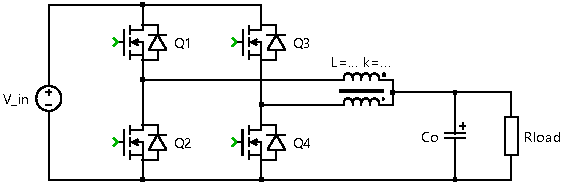
\includegraphics[width=0.85\columnwidth]{figures/Schematic_BuckConfig_Coupled.pdf}
  \caption{Schematic of the Coupled Inductor Buck Converter.}
  \label{fig:Schematic_BuckConfig_Coupled}
\end{figure}
The topology of the two phase coupled-inductor buck converter is shown in figure \ref{fig:Schematic_BuckConfig_Coupled}.
By integrating both inductors on the same core, the inductor volume can be shrunk significantly while the modulation remains the same: Both legs are switched \qty{180}{\degree} out of phase. If the ripple is more than twice the phase current, the leg current becomes negative prior to the rising edge of each leg resulting in a \ac{zvs} turn-on of all transistors. Only the small turn-off losses are observed now. This mode is called \ac{tcm} \cite{marxgutInterleavedTriangularCurrent2010}. %As the output current changes, the frequency needs to be adjusted to maintain the desired negative current.

\begin{figure}
  \begin{subfigure}[c]{\columnwidth}
      \centering
      % This file was created by matlab2tikz.
%
\definecolor{mycolor1}{rgb}{0.00000,0.44700,0.74100}%
\definecolor{mycolor2}{rgb}{0.85000,0.32500,0.09800}%
%
\begin{tikzpicture}

\begin{axis}[%
width=0.8\textwidth,
height=0.209\textwidth,
at={(0\textwidth,0.291\textwidth)},
scale only axis,
xmin=0,
xmax=1,
ymin=-2.44705852429315,
ymax=50.4066846931408,
ylabel style={font=\color{white!15!black}},
ylabel={Voltage [V]},
axis background/.style={fill=white},
axis x line*=bottom,
axis y line*=left,
xmajorgrids,
ymajorgrids,
legend style={at={(0.03,0.97)}, anchor=north west, legend cell align=left, align=left, draw=white!15!black}
]
\addplot [color=mycolor1]
  table[row sep=crcr]{%
0	0.00472205805341957\\
0.0001	4.73103698409356\\
0.0002	9.4639203911674\\
0.001	47.2167083475145\\
0.00101674718245128	47.9999999999984\\
0.00101674718245137	48.0000000000028\\
0.00338802201804276	48.0041977332192\\
0.00793312257787043	48.0032961840595\\
0.00999999999999972	48.002885939654\\
0.01	48.002885939654\\
0.0463608044786215	47.9956709336595\\
0.249999999999995	47.9553560205539\\
0.250000000000005	47.9553560205539\\
0.250107397585656	8.98126018000767e-12\\
0.250107397585663	-3.15844772558194e-09\\
0.250390458970142	-0.0445742700339777\\
0.250447071247038	-0.0446156507734269\\
0.250736732374929	-0.0445882035888449\\
0.253054021398058	-0.0443666992909175\\
0.259999999999997	-0.0437028119133129\\
0.260000000000005	-0.0437028119133122\\
0.278538312185035	-0.0419314434703845\\
0.426844809665279	-0.0277972771196984\\
0.499999999999986	-0.0208589676321533\\
0.5	-0.020858967632152\\
0.5004	-0.0208280474518644\\
0.5008	-0.0208110216106691\\
0.501014807882517	-0.0208074770476585\\
0.501014807882531	-0.0208074770476584\\
0.503207934999303	-0.0207926962238433\\
0.507409638361051	-0.0207643578281453\\
0.509999999999985	-0.0207468732973994\\
0.51	-0.0207468732973993\\
0.543613626893986	-0.0205189049022681\\
0.749999999999988	-0.0190453446354113\\
0.750000000000012	-0.0190453446354112\\
0.750107417849607	-0.0190399949401235\\
0.750107417849628	-0.0190399949401215\\
0.750390492993177	-0.0190129668133518\\
0.750447108021887	-0.0190075611410194\\
0.750736800362785	-0.0189799010630864\\
0.753054339089966	-0.018758626261391\\
0.75999999999999	-0.0180955293633729\\
0.760000000000012	-0.0180955293633708\\
0.778540309817458	-0.0163259990200823\\
0.926862788357029	-0.00220654014408546\\
0.999999999999972	0.00472206417992121\\
1	0.00472206417992389\\
};
\addlegendentry{$\text{V}_{\text{leg1}}$}

\addplot [color=mycolor2]
  table[row sep=crcr]{%
0	-0.020850567247542\\
0.0001	-0.0208415329320944\\
0.0002	-0.0208333658890972\\
0.001	-0.0207992177429933\\
0.00101674718245128	-0.020799077933846\\
0.00101674718245137	-0.020799077933846\\
0.00338802201804276	-0.0207830962457764\\
0.00793312257787043	-0.0207524394771466\\
0.00999999999999972	-0.0207384875863653\\
0.01	-0.0207384875863653\\
0.0463608044786215	-0.0204917907883527\\
0.249999999999995	-0.0190369653440986\\
0.250000000000005	-0.0190369653440985\\
0.250107397585656	-0.019031616682487\\
0.250107397585663	-0.0190316166824863\\
0.250390458970142	-0.019004589872909\\
0.250447071247038	-0.0189991844685229\\
0.250736732374929	-0.0189715273779559\\
0.253054021398058	-0.018750276510175\\
0.259999999999997	-0.0180871495110683\\
0.260000000000005	-0.0180871495110676\\
0.278538312185035	-0.0163178103558459\\
0.426844809665279	-0.00219987244712331\\
0.499999999999986	0.0047304357508528\\
0.5	0.00473043575085414\\
0.5004	18.9712942321575\\
0.5008	37.9038862369509\\
0.501014807882517	47.9999999996636\\
0.501014807882531	48.0000000003374\\
0.503207934999303	48.0042418196211\\
0.507409638361051	48.0034085385727\\
0.509999999999985	48.0028943990834\\
0.51	48.0028943990834\\
0.543613626893986	47.996224346614\\
0.749999999999988	47.9553647792131\\
0.750000000000012	47.9553647792131\\
0.750107417849607	4.76006789540406e-09\\
0.750107417849628	-4.78792117064586e-09\\
0.750390492993177	-0.044565864877198\\
0.750447108021887	-0.0446072342825728\\
0.750736800362785	-0.0445797840594028\\
0.753054339089966	-0.0443582559660125\\
0.75999999999999	-0.0436943992244668\\
0.760000000000012	-0.0436943992244648\\
0.778540309817458	-0.0419228407080231\\
0.926862788357029	-0.0277871622370406\\
0.999999999999972	-0.0208505638780304\\
1	-0.0208505638780277\\
};
\addlegendentry{$\text{V}_{\text{leg2}}$}

\end{axis}

\begin{axis}[%
width=0.8\textwidth,
height=0.209\textwidth,
at={(0\textwidth,0\textwidth)},
scale only axis,
xmin=0,
xmax=1,
xlabel style={font=\color{white!15!black}},
xlabel={$\text{Time [}\mu\text{s]}$},
ymin=-7.21478925853902,
ymax=47.1180261989237,
ylabel style={font=\color{white!15!black}},
ylabel={Current [A]},
axis background/.style={fill=white},
axis x line*=bottom,
axis y line*=left,
xmajorgrids,
ymajorgrids,
legend style={at={(0.03,0.97)}, anchor=north west, legend cell align=left, align=left, draw=white!15!black}
]
\addplot [color=mycolor1]
  table[row sep=crcr]{%
0	-4.72206849081997\\
0.0001	-4.73008044546788\\
0.0002	-4.7352047858416\\
0.001	-4.67224126477494\\
0.00101674718245128	-4.66900638413365\\
0.00101674718245137	-4.66900638413364\\
0.00338802201804276	-4.19831705149963\\
0.00793312257787043	-3.29616920074248\\
0.00999999999999972	-2.88593564861763\\
0.01	-2.88593564861757\\
0.0463608044786215	4.32908617801534\\
0.249999999999995	44.6422968333959\\
0.250000000000005	44.6422968333978\\
0.250107397585656	44.648352769039\\
0.250107397585663	44.6483527690384\\
0.250390458970142	44.62129468347\\
0.250447071247038	44.6158830795175\\
0.250736732374929	44.5881942817864\\
0.253054021398058	44.3666897156631\\
0.259999999999997	43.702802356147\\
0.260000000000005	43.7028023561462\\
0.278538312185035	41.9314339867277\\
0.426844809665279	27.797267500686\\
0.499999999999986	20.8589580708964\\
0.5	20.8589580708951\\
0.5004	20.8280414596057\\
0.5008	20.8110190862577\\
0.501014807882517	20.8074763725119\\
0.501014807882531	20.8074763725118\\
0.503207934999303	20.7926955558395\\
0.507409638361051	20.7643571638653\\
0.509999999999985	20.746872608273\\
0.51	20.7468726082729\\
0.543613626893986	20.5189042207751\\
0.749999999999988	19.0453445886524\\
0.750000000000012	19.0453445886522\\
0.750107417849607	19.0399857006543\\
0.750107417849628	19.0399857006523\\
0.750390492993177	19.0129572642142\\
0.750447108021887	19.0075515930781\\
0.750736800362785	18.979891515272\\
0.753054339089966	18.7586167083359\\
0.75999999999999	18.0955198206555\\
0.760000000000012	18.0955198206534\\
0.778540309817458	16.3259894779239\\
0.926862788357029	2.20653074668054\\
0.999999999999972	-4.72207360050509\\
1	-4.72207360050777\\
};
\addlegendentry{$\text{I}_\text{1}$}

\addplot [color=mycolor2]
  table[row sep=crcr]{%
0	20.8505568211645\\
0.0001	20.8415243288634\\
0.0002	20.8333581552167\\
0.001	20.7992169234678\\
0.00101674718245128	20.7990772577733\\
0.00101674718245137	20.7990772577733\\
0.00338802201804276	20.7830955655879\\
0.00793312257787043	20.7524388194549\\
0.00999999999999972	20.7384869226217\\
0.01	20.7384869226217\\
0.0463608044786215	20.4917901062744\\
0.249999999999995	19.0369652996204\\
0.250000000000005	19.0369652996204\\
0.250107397585656	19.0316074440422\\
0.250107397585663	19.0316074440415\\
0.250390458970142	19.0045803270553\\
0.250447071247038	18.9991749206063\\
0.250736732374929	18.9715178329643\\
0.253054021398058	18.7502669461409\\
0.259999999999997	18.0871399648492\\
0.260000000000005	18.0871399648485\\
0.278538312185035	16.3178008791562\\
0.426844809665279	2.19986287662209\\
0.499999999999986	-4.73044531151799\\
0.5	-4.73044531151934\\
0.5004	-4.74511582865435\\
0.5008	-4.71347331089969\\
0.501014807882517	-4.67781868058654\\
0.501014807882531	-4.67781868058369\\
0.503207934999303	-4.24249047004786\\
0.507409638361051	-3.4084991017942\\
0.509999999999985	-2.89436271212499\\
0.51	-2.89436271212211\\
0.543613626893986	3.77567322461342\\
0.749999999999988	44.6338807485354\\
0.750000000000012	44.63388074854\\
0.750107417849607	44.6399377711357\\
0.750107417849628	44.6399377711337\\
0.750390492993177	44.6128783849188\\
0.750447108021887	44.6074665200409\\
0.750736800362785	44.5797747495187\\
0.753054339089966	44.3582464022666\\
0.75999999999999	43.694389669589\\
0.760000000000012	43.6943896695869\\
0.778540309817458	41.9228311549258\\
0.926862788357029	27.7871528320079\\
0.999999999999972	20.8505544538598\\
1	20.8505544538571\\
};
\addlegendentry{$\text{I}_\text{2}$}

\end{axis}
\end{tikzpicture}%
      \subcaption{Negative Coupling (\sbl{k} = -0.3)}
      \label{fig:waveform_negCoupling}
    \end{subfigure}
    \begin{subfigure}[c]{\columnwidth}
      \centering
      % This file was created by matlab2tikz.
%
\definecolor{mycolor1}{rgb}{0.00000,0.44700,0.74100}%
\definecolor{mycolor2}{rgb}{0.85000,0.32500,0.09800}%
%
\begin{tikzpicture}

\begin{axis}[%
width=0.8\textwidth,
height=0.209\textwidth,
at={(0\textwidth,0.291\textwidth)},
scale only axis,
xmin=0,
xmax=1,
ymin=-2.44585469933321,
ymax=50.405429669023,
ylabel style={font=\color{white!15!black}},
ylabel={Voltage [V]},
axis background/.style={fill=white},
axis x line*=bottom,
axis y line*=left,
xmajorgrids,
ymajorgrids,
legend style={at={(0.03,0.97)}, anchor=north west, legend cell align=left, align=left, draw=white!15!black}
]
\addplot [color=mycolor1]
  table[row sep=crcr]{%
0	0.00364915155723571\\
0.0001	3.65450596530095\\
0.0002	7.30760222271523\\
0.001	36.4037137920013\\
0.00132395218332397	47.9999999999987\\
0.00132395218332407	48.0000000000022\\
0.00377322162316277	48.0030851511827\\
0.00880074145349935	48.0021329019186\\
0.00999999999999972	48.0019057123886\\
0.01	48.0019057123886\\
0.0502201586426926	47.9942858607021\\
0.249999999999995	47.9564723232359\\
0.250000000000005	47.9564723232359\\
0.250110150220581	1.54261670104461e-09\\
0.250110150220588	-1.59207047545351e-09\\
0.250411309667228	-0.0434810892693542\\
0.250471541556556	-0.0435215790524895\\
0.250786377612408	-0.0435091199836403\\
0.25330506605922	-0.0434077800409767\\
0.259999999999998	-0.043138418230516\\
0.260000000000005	-0.0431384182305157\\
0.280149507574504	-0.0423278309126668\\
0.441345568170493	-0.0358510373540963\\
0.499999999999986	-0.0334991709947935\\
0.5	-0.0334991709947929\\
0.5004	-0.0334789608517999\\
0.5008	-0.0334503896158805\\
0.501325069396783	-0.0334003748522959\\
0.501325069396797	-0.0334003748522943\\
0.503687467527966	-0.0331431844576095\\
0.508537742459238	-0.0326151530914254\\
0.509999999999985	-0.0324559651882885\\
0.51	-0.032455965188287\\
0.548802199450177	-0.0282321972960459\\
0.749999999999988	-0.00633865264511624\\
0.750000000000012	-0.00633865264511359\\
0.750110140154645	-0.00633028778078904\\
0.750110140154666	-0.00633028778078816\\
0.750431371446163	-0.00631743697375792\\
0.750495617704463	-0.00631486681947\\
0.750836750924163	-0.00630121990016192\\
0.753565816681768	-0.00619204597008259\\
0.759999999999991	-0.00593466226564735\\
0.760000000000012	-0.00593466226564648\\
0.781832526060849	-0.00506142151177709\\
0.956492734547545	0.00191499525219897\\
0.999999999999972	0.0036491671660061\\
1	0.00364916716600723\\
};
\addlegendentry{$\text{V}_{\text{leg1}}$}

\addplot [color=mycolor2]
  table[row sep=crcr]{%
0	-0.033502118923243\\
0.0001	-0.0334978509045324\\
0.0002	-0.0334930594226207\\
0.001	-0.0334359116753486\\
0.00132395218332397	-0.0334034228283609\\
0.00132395218332407	-0.0334034228283608\\
0.00377322162316277	-0.0331367749049176\\
0.00880074145349935	-0.0325894479556535\\
0.00999999999999972	-0.0324588913695065\\
0.01	-0.0324588913695065\\
0.0502201586426926	-0.0280807863647854\\
0.249999999999995	-0.00634157413732197\\
0.250000000000005	-0.00634157413732082\\
0.250110150220581	-0.00633323928411055\\
0.250110150220588	-0.00633323928411026\\
0.250411309667228	-0.00632119143732688\\
0.250471541556556	-0.00631878187511698\\
0.250786377612408	-0.00630618695600671\\
0.25330506605922	-0.0062054288146152\\
0.259999999999998	-0.00593761397402845\\
0.260000000000005	-0.00593761397402815\\
0.280149507574504	-0.00513168212841396\\
0.441345568170493	0.0013078886278803\\
0.499999999999986	0.00364621994593294\\
0.5	0.00364621994593351\\
0.5004	14.6018175772046\\
0.5008	29.1521646289979\\
0.501325069396783	47.9999999997474\\
0.501325069396797	48.000000000258\\
0.503687467527966	48.0030985613705\\
0.508537742459238	48.0021798825724\\
0.509999999999985	48.0019028638981\\
0.51	48.0019028638981\\
0.548802199450177	47.9945508749325\\
0.749999999999988	47.9564694758343\\
0.750000000000012	47.9564694758343\\
0.750110140154645	2.72848410531878e-12\\
0.750110140154666	-9.30981514102314e-09\\
0.750431371446163	-0.0434859161360918\\
0.750495617704463	-0.0435235916806508\\
0.750836750924163	-0.043510049682441\\
0.753565816681768	-0.0434002452023034\\
0.759999999999991	-0.0431413745437156\\
0.760000000000012	-0.0431413745437147\\
0.781832526060849	-0.0422630886860356\\
0.956492734547545	-0.0352463357228472\\
0.999999999999972	-0.0335021230109665\\
1	-0.0335021230109653\\
};
\addlegendentry{$\text{V}_{\text{leg2}}$}

\end{axis}

\begin{axis}[%
width=0.8\textwidth,
height=0.209\textwidth,
at={(0\textwidth,0\textwidth)},
scale only axis,
xmin=0,
xmax=1,
xlabel style={font=\color{white!15!black}},
xlabel={$\text{Time [}\mu\text{s]}$},
ymin=-6.01328004382146,
ymax=45.8989273840632,
ylabel style={font=\color{white!15!black}},
ylabel={Current [A]},
axis background/.style={fill=white},
axis x line*=bottom,
axis y line*=left,
xmajorgrids,
ymajorgrids,
legend style={at={(0.03,0.97)}, anchor=north west, legend cell align=left, align=left, draw=white!15!black}
]
\addplot [color=mycolor1]
  table[row sep=crcr]{%
0	-3.64915554245843\\
0.0001	-3.65226736182266\\
0.0002	-3.65363425164488\\
0.001	-3.60184866888934\\
0.00132395218332397	-3.54972024010614\\
0.00132395218332407	-3.54972024010612\\
0.00377322162316277	-3.08559452310081\\
0.00880074145349935	-2.13292575824823\\
0.00999999999999972	-1.90568208920071\\
0.01	-1.90568208920065\\
0.0502201586426926	5.7144033049679\\
0.249999999999995	43.5276852632097\\
0.250000000000005	43.5276852632117\\
0.250110150220581	43.5363247054634\\
0.250110150220588	43.5363247054631\\
0.250411309667228	43.5242073077433\\
0.250471541556556	43.5217838276639\\
0.250786377612408	43.5091161573977\\
0.25330506605922	43.4077760110589\\
0.259999999999998	43.1384142072457\\
0.260000000000005	43.1384142072454\\
0.280149507574504	42.3278268902044\\
0.441345568170493	35.8510331565057\\
0.499999999999986	33.4991668764244\\
0.5	33.4991668764239\\
0.5004	33.4789547528307\\
0.5008	33.4503814308296\\
0.501325069396783	33.4003639665544\\
0.501325069396797	33.4003639665528\\
0.503687467527966	33.1431735681184\\
0.508537742459238	32.6151422063661\\
0.509999999999985	32.4559543028131\\
0.51	32.4559543028116\\
0.548802199450177	28.2321864626815\\
0.749999999999988	6.33864176483613\\
0.750000000000012	6.33864176483348\\
0.750110140154645	6.33028377085221\\
0.750110140154666	6.33028377085133\\
0.750431371446163	6.31743297321812\\
0.750495617704463	6.31486281901573\\
0.750836750924163	6.30121590006242\\
0.753565816681768	6.19204197103698\\
0.759999999999991	5.93465825797117\\
0.760000000000012	5.93465825797031\\
0.781832526060849	5.06141746183346\\
0.956492734547545	-1.91499924013165\\
0.999999999999972	-3.64917120830515\\
1	-3.64917120830628\\
};
\addlegendentry{$\text{I}_\text{1}$}

\addplot [color=mycolor2]
  table[row sep=crcr]{%
0	33.5021149137854\\
0.0001	33.4978463749054\\
0.0002	33.4930543694835\\
0.001	33.4359024510314\\
0.00132395218332397	33.4034119424097\\
0.00132395218332407	33.4034119424097\\
0.00377322162316277	33.1367640226971\\
0.00880074145349935	32.5894370775034\\
0.00999999999999972	32.4588804890695\\
0.01	32.4588804890695\\
0.0502201586426926	28.0807756345671\\
0.249999999999995	6.34156325020789\\
0.250000000000005	6.34156325020674\\
0.250110150220581	6.33323527110644\\
0.250110150220588	6.33323527110614\\
0.250411309667228	6.321187436763\\
0.250471541556556	6.31877787471868\\
0.250786377612408	6.30618295499368\\
0.25330506605922	6.20542480786427\\
0.259999999999998	5.93760997377455\\
0.260000000000005	5.93760997377425\\
0.280149507574504	5.13167812905479\\
0.441345568170493	-1.30789279377418\\
0.499999999999986	-3.64622404965078\\
0.5	-3.64622404965135\\
0.5004	-3.64821117971264\\
0.5008	-3.62232714166394\\
0.501325069396783	-3.54664928738605\\
0.501325069396797	-3.54664928738332\\
0.503687467527966	-3.0989852129238\\
0.508537742459238	-2.17990172700418\\
0.509999999999985	-1.90282299690865\\
0.51	-1.9028229969059\\
0.548802199450177	5.44865344881221\\
0.749999999999988	43.530540349799\\
0.750000000000012	43.5305403498036\\
0.750110140154645	43.5392815918867\\
0.750110140154666	43.5392815918859\\
0.750431371446163	43.5263565809959\\
0.750495617704463	43.5237715787822\\
0.750836750924163	43.5100458201866\\
0.753565816681768	43.4002411800356\\
0.759999999999991	43.1413705128681\\
0.760000000000012	43.1413705128672\\
0.781832526060849	42.2630846142092\\
0.956492734547545	35.2463317118329\\
0.999999999999972	33.5021189387663\\
1	33.5021189387651\\
};
\addlegendentry{$\text{I}_\text{2}$}

\end{axis}
\end{tikzpicture}%
      \subcaption{Positive Coupling (\sbl{k} = 0.3)}
      \label{fig:waveform_posCoupling}
    \end{subfigure}
  \caption{Waveforms for positive and negative coupling. It can be seen that the slopes are changed but the behavior in the vicinity of the switching instances is fundamentally the same. ToDo: Make smaller!}
  \label{fig:waveform_Coupling}
\end{figure}

\subsection{Impact of the Coupling Factor}
The symmetrical coupled inductor consists of two identical coils that are wound in a way, that the flux of one coil links with the flux of the second coil and vice versa with both coils connected on one side. This configuration can be described mathematically using 
\begin{equation}
  \label{eq:StandardCoupling}
  \begin{bmatrix} v_\mathrm a \\ v_\mathrm b \end{bmatrix} = \begin{bmatrix} 1 & \sbl{k} \\ \sbl{k} & 1 \end{bmatrix} \sbl{Lself} \begin{bmatrix} \frac{d\sbl{i1}}{dt}  \\ \frac{d\sbl{i2}}{dt} \end{bmatrix}
\end{equation}
with self-inductance \sbl{Lself} and coupling-factor \sbl{k}. Note that \sbl{k} can be positive or negative; the impact of that will be analyzed later.
In order to simplify the equations and provide a more intuitive understanding, the equivalent circuit in figure TODO is introduced. Both circuits are electrically equivalent for
\begin{equation}
  \label{eq:LoutandLmfromk}
  \begin{aligned}
    \sbl{Lout} & = (1+\sbl{k})\frac{\sbl{Lself}}{2} \\
    \sbl{Lm} & = (1-\sbl{k})\frac{\sbl{Lself}}{2}.
  \end{aligned}
\end{equation}
The voltage at the virtual central node is now only dependent of the two leg voltages \sbl{v1} and \sbl{v2} decoupling the governing equations:
\begin{equation}
  \label{eq:TransformerModel}
  \begin{aligned}
    \frac{d\sbl{iout}}{dt} &= \frac{1}{\sbl{Lout}} \left (\frac{\sbl{v1} + \sbl{v2}}{2}-\sbl{vout} \right ) \\
    \frac{d\sbl{im}}{dt} &= \frac{1}{\sbl{Lout}} \left (\frac{\sbl{v1} - \sbl{v2}}{2} \right ) \\
    \text{with} \quad \sbl{iout} &= \sbl{i1} + \sbl{i2} \quad \text{and} \quad \sbl{im} = \sbl{i1} - \sbl{i2}
  \end{aligned}
\end{equation}
From this, the differential equations for each interval can be easily calculated and afterwards the important converter parameters. An effective dutycycle \sbl{Deff} can be introduced with $\sbl{Deff} = D$ for $\sbl{D} \leq 0.5$ and $\sbl{Deff} = 1-D$ for $\sbl{D} > 0.5$.
The output ripple is given by
\begin{equation}
  \frac{2\sbl{Vin}}{\sbl{fs}(1+\sbl{k})\sbl{Lself}}\sbl{Deff}\left (\frac{1}{2}-\sbl{Deff} \right ).
\end{equation}
The ripple in each leg which is important for soft-switching is
\begin{equation}
  \sbl{DeltaIleg} =  \frac{\sbl{Vin}\sbl{Deff}}{2\sbl{fs}\sbl{Lself}} \left (\frac{2}{1+\sbl{k}} \left (\frac{1}{2}-\sbl{Deff} \right ) + \frac{1}{1-\sbl{k}} \right )  .
\end{equation}
Both are shown in figure \ref{fig:OutputAndLegRipple}. There is a strong dependency of these parameters with dutycycle but interestingly, the leg ripple current is not that significantly influenced by the coupling-factor. As the coupling increases, \sbl{Lout} increases while \sbl{Lm} decreases causing a decrease in \sbl{iout} but an increase in \sbl{im}.
\begin{figure}
  \centering
  % This file was created by matlab2tikz.
%
\definecolor{mycolor1}{rgb}{0.00000,0.44700,0.74100}%
\definecolor{mycolor2}{rgb}{0.85000,0.32500,0.09800}%
\definecolor{mycolor3}{rgb}{0.92900,0.69400,0.12500}%
\definecolor{mycolor4}{rgb}{0.49400,0.18400,0.55600}%
\definecolor{mycolor5}{rgb}{0.46600,0.67400,0.18800}%
\definecolor{mycolor6}{rgb}{0.30100,0.74500,0.93300}%
%
\begin{tikzpicture}

\begin{axis}[%
width=\columnwidth,
height=0.45\columnwidth,
%at={(0\columnwidth,0\columnwidth)},
%scale only axis,
xmin=0,
xmax=1,
%xlabel style={font=\color{white!15!black}},
xlabel={Dutycycle},
%x label style={at={(axis description cs:0.5,0.03)},anchor=north},
ymin=0,
ymax=13,
ytick distance = 2,
%ylabel style={font=\color{white!15!black}},
ylabel={Output current ripple [A]},
%y label style={at={(axis description cs:0.1,.5)},anchor=south},
%axis background/.style={fill=white},
%axis x line*=bottom,
%axis y line*=left,
xmajorgrids,
ymajorgrids,
%legend style={at={(0.5,-0.22)}, anchor=north, legend cell align=left, align=left, draw=white!15!black},
%legend columns=-1
%legend style={at={(1.02,0.5)}, anchor=west, legend cell align=left, align=left, draw=white!15!black},
]
\addplot [color=mycolor1, line width=1.0pt]
  table[row sep=crcr]{%
0	0\\
0.01	0.9408\\
0.02	1.8432\\
0.03	2.7072\\
0.04	3.5328\\
0.05	4.32\\
0.06	5.0688\\
0.07	5.7792\\
0.08	6.4512\\
0.09	7.0848\\
0.1	7.68\\
0.11	8.2368\\
0.12	8.7552\\
0.13	9.2352\\
0.14	9.6768\\
0.15	10.08\\
0.16	10.4448\\
0.17	10.7712\\
0.18	11.0592\\
0.19	11.3088\\
0.2	11.52\\
0.21	11.6928\\
0.22	11.8272\\
0.23	11.9232\\
0.24	11.9808\\
0.25	12\\
0.26	11.9808\\
0.27	11.9232\\
0.28	11.8272\\
0.29	11.6928\\
0.3	11.52\\
0.31	11.3088\\
0.32	11.0592\\
0.33	10.7712\\
0.34	10.4448\\
0.35	10.08\\
0.36	9.6768\\
0.37	9.2352\\
0.38	8.7552\\
0.39	8.2368\\
0.4	7.68\\
0.41	7.0848\\
0.42	6.4512\\
0.43	5.7792\\
0.44	5.0688\\
0.45	4.32\\
0.46	3.5328\\
0.47	2.7072\\
0.48	1.8432\\
0.49	0.940800000000001\\
0.5	0\\
0.51	0.940800000000001\\
0.52	1.8432\\
0.53	2.7072\\
0.54	3.5328\\
0.55	4.32\\
0.56	5.0688\\
0.57	5.7792\\
0.58	6.4512\\
0.59	7.0848\\
0.6	7.68\\
0.61	8.2368\\
0.62	8.7552\\
0.63	9.2352\\
0.64	9.6768\\
0.65	10.08\\
0.66	10.4448\\
0.67	10.7712\\
0.68	11.0592\\
0.69	11.3088\\
0.7	11.52\\
0.71	11.6928\\
0.72	11.8272\\
0.73	11.9232\\
0.74	11.9808\\
0.75	12\\
0.76	11.9808\\
0.77	11.9232\\
0.78	11.8272\\
0.79	11.6928\\
0.8	11.52\\
0.81	11.3088\\
0.82	11.0592\\
0.83	10.7712\\
0.84	10.4448\\
0.85	10.08\\
0.86	9.6768\\
0.87	9.2352\\
0.88	8.7552\\
0.89	8.2368\\
0.9	7.68\\
0.91	7.0848\\
0.92	6.4512\\
0.93	5.7792\\
0.94	5.0688\\
0.95	4.32\\
0.96	3.5328\\
0.97	2.7072\\
0.98	1.8432\\
0.99	0.940800000000001\\
1	0\\
};
\addlegendentry{k= -0.5}

\addplot [color=mycolor2, line width=1.0pt]
  table[row sep=crcr]{%
0	0\\
0.01	0.6272\\
0.02	1.2288\\
0.03	1.8048\\
0.04	2.3552\\
0.05	2.88\\
0.06	3.3792\\
0.07	3.8528\\
0.08	4.3008\\
0.09	4.7232\\
0.1	5.12\\
0.11	5.4912\\
0.12	5.8368\\
0.13	6.1568\\
0.14	6.4512\\
0.15	6.72\\
0.16	6.9632\\
0.17	7.1808\\
0.18	7.3728\\
0.19	7.5392\\
0.2	7.68\\
0.21	7.7952\\
0.22	7.8848\\
0.23	7.9488\\
0.24	7.9872\\
0.25	8\\
0.26	7.9872\\
0.27	7.9488\\
0.28	7.8848\\
0.29	7.7952\\
0.3	7.68\\
0.31	7.5392\\
0.32	7.3728\\
0.33	7.1808\\
0.34	6.9632\\
0.35	6.72\\
0.36	6.4512\\
0.37	6.1568\\
0.38	5.8368\\
0.39	5.4912\\
0.4	5.12\\
0.41	4.7232\\
0.42	4.3008\\
0.43	3.8528\\
0.44	3.3792\\
0.45	2.88\\
0.46	2.3552\\
0.47	1.8048\\
0.48	1.2288\\
0.49	0.627200000000001\\
0.5	0\\
0.51	0.627200000000001\\
0.52	1.2288\\
0.53	1.8048\\
0.54	2.3552\\
0.55	2.88\\
0.56	3.3792\\
0.57	3.8528\\
0.58	4.3008\\
0.59	4.7232\\
0.6	5.12\\
0.61	5.4912\\
0.62	5.8368\\
0.63	6.1568\\
0.64	6.4512\\
0.65	6.72\\
0.66	6.9632\\
0.67	7.1808\\
0.68	7.3728\\
0.69	7.5392\\
0.7	7.68\\
0.71	7.7952\\
0.72	7.8848\\
0.73	7.9488\\
0.74	7.9872\\
0.75	8\\
0.76	7.9872\\
0.77	7.9488\\
0.78	7.8848\\
0.79	7.7952\\
0.8	7.68\\
0.81	7.5392\\
0.82	7.3728\\
0.83	7.1808\\
0.84	6.9632\\
0.85	6.72\\
0.86	6.4512\\
0.87	6.1568\\
0.88	5.8368\\
0.89	5.4912\\
0.9	5.12\\
0.91	4.7232\\
0.92	4.3008\\
0.93	3.8528\\
0.94	3.3792\\
0.95	2.88\\
0.96	2.3552\\
0.97	1.8048\\
0.98	1.2288\\
0.99	0.627200000000001\\
1	0\\
};
\addlegendentry{k= -0.25}

\addplot [color=mycolor3, line width=1.0pt]
  table[row sep=crcr]{%
0	0\\
0.01	0.4704\\
0.02	0.9216\\
0.03	1.3536\\
0.04	1.7664\\
0.05	2.16\\
0.06	2.5344\\
0.07	2.8896\\
0.08	3.2256\\
0.09	3.5424\\
0.1	3.84\\
0.11	4.1184\\
0.12	4.3776\\
0.13	4.6176\\
0.14	4.8384\\
0.15	5.04\\
0.16	5.2224\\
0.17	5.3856\\
0.18	5.5296\\
0.19	5.6544\\
0.2	5.76\\
0.21	5.8464\\
0.22	5.9136\\
0.23	5.9616\\
0.24	5.9904\\
0.25	6\\
0.26	5.9904\\
0.27	5.9616\\
0.28	5.9136\\
0.29	5.8464\\
0.3	5.76\\
0.31	5.6544\\
0.32	5.5296\\
0.33	5.3856\\
0.34	5.2224\\
0.35	5.04\\
0.36	4.8384\\
0.37	4.6176\\
0.38	4.3776\\
0.39	4.1184\\
0.4	3.84\\
0.41	3.5424\\
0.42	3.2256\\
0.43	2.8896\\
0.44	2.5344\\
0.45	2.16\\
0.46	1.7664\\
0.47	1.3536\\
0.48	0.921600000000001\\
0.49	0.4704\\
0.5	0\\
0.51	0.4704\\
0.52	0.921600000000001\\
0.53	1.3536\\
0.54	1.7664\\
0.55	2.16\\
0.56	2.5344\\
0.57	2.8896\\
0.58	3.2256\\
0.59	3.5424\\
0.6	3.84\\
0.61	4.1184\\
0.62	4.3776\\
0.63	4.6176\\
0.64	4.8384\\
0.65	5.04\\
0.66	5.2224\\
0.67	5.3856\\
0.68	5.5296\\
0.69	5.6544\\
0.7	5.76\\
0.71	5.8464\\
0.72	5.9136\\
0.73	5.9616\\
0.74	5.9904\\
0.75	6\\
0.76	5.9904\\
0.77	5.9616\\
0.78	5.9136\\
0.79	5.8464\\
0.8	5.76\\
0.81	5.6544\\
0.82	5.5296\\
0.83	5.3856\\
0.84	5.2224\\
0.85	5.04\\
0.86	4.8384\\
0.87	4.6176\\
0.88	4.3776\\
0.89	4.1184\\
0.9	3.84\\
0.91	3.5424\\
0.92	3.2256\\
0.93	2.8896\\
0.94	2.5344\\
0.95	2.16\\
0.96	1.7664\\
0.97	1.3536\\
0.98	0.921600000000001\\
0.99	0.4704\\
1	0\\
};
\addlegendentry{k= 0}

\addplot [color=mycolor4, line width=1.0pt]
  table[row sep=crcr]{%
0	0\\
0.01	0.37632\\
0.02	0.73728\\
0.03	1.08288\\
0.04	1.41312\\
0.05	1.728\\
0.06	2.02752\\
0.07	2.31168\\
0.08	2.58048\\
0.09	2.83392\\
0.1	3.072\\
0.11	3.29472\\
0.12	3.50208\\
0.13	3.69408\\
0.14	3.87072\\
0.15	4.032\\
0.16	4.17792\\
0.17	4.30848\\
0.18	4.42368\\
0.19	4.52352\\
0.2	4.608\\
0.21	4.67712\\
0.22	4.73088\\
0.23	4.76928\\
0.24	4.79232\\
0.25	4.8\\
0.26	4.79232\\
0.27	4.76928\\
0.28	4.73088\\
0.29	4.67712\\
0.3	4.608\\
0.31	4.52352\\
0.32	4.42368\\
0.33	4.30848\\
0.34	4.17792\\
0.35	4.032\\
0.36	3.87072\\
0.37	3.69408\\
0.38	3.50208\\
0.39	3.29472\\
0.4	3.072\\
0.41	2.83392\\
0.42	2.58048\\
0.43	2.31168\\
0.44	2.02752\\
0.45	1.728\\
0.46	1.41312\\
0.47	1.08288\\
0.48	0.737280000000001\\
0.49	0.37632\\
0.5	0\\
0.51	0.37632\\
0.52	0.737280000000001\\
0.53	1.08288\\
0.54	1.41312\\
0.55	1.728\\
0.56	2.02752\\
0.57	2.31168\\
0.58	2.58048\\
0.59	2.83392\\
0.6	3.072\\
0.61	3.29472\\
0.62	3.50208\\
0.63	3.69408\\
0.64	3.87072\\
0.65	4.032\\
0.66	4.17792\\
0.67	4.30848\\
0.68	4.42368\\
0.69	4.52352\\
0.7	4.608\\
0.71	4.67712\\
0.72	4.73088\\
0.73	4.76928\\
0.74	4.79232\\
0.75	4.8\\
0.76	4.79232\\
0.77	4.76928\\
0.78	4.73088\\
0.79	4.67712\\
0.8	4.608\\
0.81	4.52352\\
0.82	4.42368\\
0.83	4.30848\\
0.84	4.17792\\
0.85	4.032\\
0.86	3.87072\\
0.87	3.69408\\
0.88	3.50208\\
0.89	3.29472\\
0.9	3.072\\
0.91	2.83392\\
0.92	2.58048\\
0.93	2.31168\\
0.94	2.02752\\
0.95	1.728\\
0.96	1.41312\\
0.97	1.08288\\
0.98	0.737280000000001\\
0.99	0.37632\\
1	0\\
};
\addlegendentry{k= 0.25}

\addplot [color=mycolor5, line width=1.0pt]
  table[row sep=crcr]{%
0	0\\
0.01	0.3136\\
0.02	0.6144\\
0.03	0.9024\\
0.04	1.1776\\
0.05	1.44\\
0.06	1.6896\\
0.07	1.9264\\
0.08	2.1504\\
0.09	2.3616\\
0.1	2.56\\
0.11	2.7456\\
0.12	2.9184\\
0.13	3.0784\\
0.14	3.2256\\
0.15	3.36\\
0.16	3.4816\\
0.17	3.5904\\
0.18	3.6864\\
0.19	3.7696\\
0.2	3.84\\
0.21	3.8976\\
0.22	3.9424\\
0.23	3.9744\\
0.24	3.9936\\
0.25	4\\
0.26	3.9936\\
0.27	3.9744\\
0.28	3.9424\\
0.29	3.8976\\
0.3	3.84\\
0.31	3.7696\\
0.32	3.6864\\
0.33	3.5904\\
0.34	3.4816\\
0.35	3.36\\
0.36	3.2256\\
0.37	3.0784\\
0.38	2.9184\\
0.39	2.7456\\
0.4	2.56\\
0.41	2.3616\\
0.42	2.1504\\
0.43	1.9264\\
0.44	1.6896\\
0.45	1.44\\
0.46	1.1776\\
0.47	0.902400000000001\\
0.48	0.614400000000001\\
0.49	0.3136\\
0.5	0\\
0.51	0.3136\\
0.52	0.614400000000001\\
0.53	0.902400000000001\\
0.54	1.1776\\
0.55	1.44\\
0.56	1.6896\\
0.57	1.9264\\
0.58	2.1504\\
0.59	2.3616\\
0.6	2.56\\
0.61	2.7456\\
0.62	2.9184\\
0.63	3.0784\\
0.64	3.2256\\
0.65	3.36\\
0.66	3.4816\\
0.67	3.5904\\
0.68	3.6864\\
0.69	3.7696\\
0.7	3.84\\
0.71	3.8976\\
0.72	3.9424\\
0.73	3.9744\\
0.74	3.9936\\
0.75	4\\
0.76	3.9936\\
0.77	3.9744\\
0.78	3.9424\\
0.79	3.8976\\
0.8	3.84\\
0.81	3.7696\\
0.82	3.6864\\
0.83	3.5904\\
0.84	3.4816\\
0.85	3.36\\
0.86	3.2256\\
0.87	3.0784\\
0.88	2.9184\\
0.89	2.7456\\
0.9	2.56\\
0.91	2.3616\\
0.92	2.1504\\
0.93	1.9264\\
0.94	1.6896\\
0.95	1.44\\
0.96	1.1776\\
0.97	0.902400000000001\\
0.98	0.614400000000001\\
0.99	0.3136\\
1	0\\
};
\addlegendentry{k= 0.5}

\addplot [color=mycolor6, dashed, line width=2.0pt]
  table[row sep=crcr]{%
0	0\\
0.01	0.4752\\
0.02	0.9408\\
0.03	1.3968\\
0.04	1.8432\\
0.05	2.28\\
0.06	2.7072\\
0.07	3.1248\\
0.08	3.5328\\
0.09	3.9312\\
0.1	4.32\\
0.11	4.6992\\
0.12	5.0688\\
0.13	5.4288\\
0.14	5.7792\\
0.15	6.12\\
0.16	6.4512\\
0.17	6.7728\\
0.18	7.0848\\
0.19	7.3872\\
0.2	7.68\\
0.21	7.9632\\
0.22	8.2368\\
0.23	8.5008\\
0.24	8.7552\\
0.25	9\\
0.26	9.2352\\
0.27	9.4608\\
0.28	9.6768\\
0.29	9.8832\\
0.3	10.08\\
0.31	10.2672\\
0.32	10.4448\\
0.33	10.6128\\
0.34	10.7712\\
0.35	10.92\\
0.36	11.0592\\
0.37	11.1888\\
0.38	11.3088\\
0.39	11.4192\\
0.4	11.52\\
0.41	11.6112\\
0.42	11.6928\\
0.43	11.7648\\
0.44	11.8272\\
0.45	11.88\\
0.46	11.9232\\
0.47	11.9568\\
0.48	11.9808\\
0.49	11.9952\\
0.5	12\\
0.51	11.9952\\
0.52	11.9808\\
0.53	11.9568\\
0.54	11.9232\\
0.55	11.88\\
0.56	11.8272\\
0.57	11.7648\\
0.58	11.6928\\
0.59	11.6112\\
0.6	11.52\\
0.61	11.4192\\
0.62	11.3088\\
0.63	11.1888\\
0.64	11.0592\\
0.65	10.92\\
0.66	10.7712\\
0.67	10.6128\\
0.68	10.4448\\
0.69	10.2672\\
0.7	10.08\\
0.71	9.8832\\
0.72	9.6768\\
0.73	9.4608\\
0.74	9.2352\\
0.75	9\\
0.76	8.7552\\
0.77	8.5008\\
0.78	8.2368\\
0.79	7.9632\\
0.8	7.68\\
0.81	7.3872\\
0.82	7.0848\\
0.83	6.7728\\
0.84	6.4512\\
0.85	6.12\\
0.86	5.7792\\
0.87	5.4288\\
0.88	5.0688\\
0.89	4.6992\\
0.9	4.32\\
0.91	3.9312\\
0.92	3.5328\\
0.93	3.1248\\
0.94	2.7072\\
0.95	2.28\\
0.96	1.8432\\
0.97	1.3968\\
0.98	0.940800000000001\\
0.99	0.4752\\
1	0\\
};
\addlegendentry{1-ph}
\legend{}

\end{axis}
\end{tikzpicture}%
  % This file was created by matlab2tikz.
%
\definecolor{mycolor1}{rgb}{0.00000,0.44700,0.74100}%
\definecolor{mycolor2}{rgb}{0.85000,0.32500,0.09800}%
\definecolor{mycolor3}{rgb}{0.92900,0.69400,0.12500}%
\definecolor{mycolor4}{rgb}{0.49400,0.18400,0.55600}%
\definecolor{mycolor5}{rgb}{0.46600,0.67400,0.18800}%
\definecolor{mycolor6}{rgb}{0.30100,0.74500,0.93300}%
%
\begin{tikzpicture}

\begin{axis}[%
width=\columnwidth,
height=0.6\columnwidth,
%at={(0\columnwidth,0\columnwidth)},
xmin=0,
xmax=1,
%xlabel style={font=\color{white!15!black}},
xlabel={Dutycycle},
%x label style={at={(axis description cs:0.5,0.03)},anchor=north},
ymin=0,
ymax=25,
ytick distance = 5,
%ylabel style={font=\color{white!15!black}},
ylabel={Leg current ripple [A]},
%y label style={at={(axis description cs:0.1,.5)},anchor=south},
%axis background/.style={fill=white},
%axis x line*=bottom,
%axis y line*=left,
xmajorgrids,
ymajorgrids,
%legend style={at={(1.02,0.5)}, anchor=west, legend cell align=left, align=left, draw=white!15!black},
legend style={at={(0.5,-0.3)}, anchor=north, legend cell align=left, align=left, draw=white!15!black},
legend columns=3
]
\addplot [color=mycolor1]
  table[row sep=crcr]{%
0	0\\
0.01	0.6304\\
0.02	1.2416\\
0.03	1.8336\\
0.04	2.4064\\
0.05	2.96\\
0.06	3.4944\\
0.07	4.0096\\
0.08	4.5056\\
0.09	4.9824\\
0.1	5.44\\
0.11	5.8784\\
0.12	6.2976\\
0.13	6.6976\\
0.14	7.0784\\
0.15	7.44\\
0.16	7.7824\\
0.17	8.1056\\
0.18	8.4096\\
0.19	8.6944\\
0.2	8.96\\
0.21	9.2064\\
0.22	9.4336\\
0.23	9.6416\\
0.24	9.8304\\
0.25	10\\
0.26	10.1504\\
0.27	10.2816\\
0.28	10.3936\\
0.29	10.4864\\
0.3	10.56\\
0.31	10.6144\\
0.32	10.6496\\
0.33	10.6656\\
0.34	10.6624\\
0.35	10.64\\
0.36	10.5984\\
0.37	10.5376\\
0.38	10.4576\\
0.39	10.3584\\
0.4	10.24\\
0.41	10.1024\\
0.42	9.9456\\
0.43	9.7696\\
0.44	9.5744\\
0.45	9.36\\
0.46	9.1264\\
0.47	8.8736\\
0.48	8.6016\\
0.49	8.3104\\
0.5	8\\
0.51	8.3104\\
0.52	8.6016\\
0.53	8.8736\\
0.54	9.1264\\
0.55	9.36\\
0.56	9.5744\\
0.57	9.7696\\
0.58	9.9456\\
0.59	10.1024\\
0.6	10.24\\
0.61	10.3584\\
0.62	10.4576\\
0.63	10.5376\\
0.64	10.5984\\
0.65	10.64\\
0.66	10.6624\\
0.67	10.6656\\
0.68	10.6496\\
0.69	10.6144\\
0.7	10.56\\
0.71	10.4864\\
0.72	10.3936\\
0.73	10.2816\\
0.74	10.1504\\
0.75	10\\
0.76	9.8304\\
0.77	9.6416\\
0.78	9.4336\\
0.79	9.2064\\
0.8	8.96\\
0.81	8.6944\\
0.82	8.4096\\
0.83	8.1056\\
0.84	7.7824\\
0.85	7.44\\
0.86	7.0784\\
0.87	6.6976\\
0.88	6.2976\\
0.89	5.8784\\
0.9	5.44\\
0.91	4.9824\\
0.92	4.5056\\
0.93	4.0096\\
0.94	3.4944\\
0.95	2.96\\
0.96	2.4064\\
0.97	1.8336\\
0.98	1.2416\\
0.99	0.630400000000001\\
1	0\\
};
\addlegendentry{k= -0.5}

\addplot [color=mycolor2]
  table[row sep=crcr]{%
0	0\\
0.01	0.5056\\
0.02	0.9984\\
0.03	1.4784\\
0.04	1.9456\\
0.05	2.4\\
0.06	2.8416\\
0.07	3.2704\\
0.08	3.6864\\
0.09	4.0896\\
0.1	4.48\\
0.11	4.8576\\
0.12	5.2224\\
0.13	5.5744\\
0.14	5.9136\\
0.15	6.24\\
0.16	6.5536\\
0.17	6.8544\\
0.18	7.1424\\
0.19	7.4176\\
0.2	7.68\\
0.21	7.9296\\
0.22	8.1664\\
0.23	8.3904\\
0.24	8.6016\\
0.25	8.8\\
0.26	8.9856\\
0.27	9.1584\\
0.28	9.3184\\
0.29	9.4656\\
0.3	9.6\\
0.31	9.7216\\
0.32	9.8304\\
0.33	9.9264\\
0.34	10.0096\\
0.35	10.08\\
0.36	10.1376\\
0.37	10.1824\\
0.38	10.2144\\
0.39	10.2336\\
0.4	10.24\\
0.41	10.2336\\
0.42	10.2144\\
0.43	10.1824\\
0.44	10.1376\\
0.45	10.08\\
0.46	10.0096\\
0.47	9.9264\\
0.48	9.8304\\
0.49	9.7216\\
0.5	9.6\\
0.51	9.7216\\
0.52	9.8304\\
0.53	9.9264\\
0.54	10.0096\\
0.55	10.08\\
0.56	10.1376\\
0.57	10.1824\\
0.58	10.2144\\
0.59	10.2336\\
0.6	10.24\\
0.61	10.2336\\
0.62	10.2144\\
0.63	10.1824\\
0.64	10.1376\\
0.65	10.08\\
0.66	10.0096\\
0.67	9.9264\\
0.68	9.8304\\
0.69	9.7216\\
0.7	9.6\\
0.71	9.4656\\
0.72	9.3184\\
0.73	9.1584\\
0.74	8.9856\\
0.75	8.8\\
0.76	8.6016\\
0.77	8.3904\\
0.78	8.1664\\
0.79	7.9296\\
0.8	7.68\\
0.81	7.4176\\
0.82	7.1424\\
0.83	6.8544\\
0.84	6.5536\\
0.85	6.24\\
0.86	5.9136\\
0.87	5.5744\\
0.88	5.2224\\
0.89	4.8576\\
0.9	4.48\\
0.91	4.0896\\
0.92	3.6864\\
0.93	3.2704\\
0.94	2.8416\\
0.95	2.4\\
0.96	1.9456\\
0.97	1.4784\\
0.98	0.998400000000001\\
0.99	0.5056\\
1	0\\
};
\addlegendentry{k= -0.25}

\addplot [color=mycolor3]
  table[row sep=crcr]{%
0	0\\
0.01	0.4752\\
0.02	0.9408\\
0.03	1.3968\\
0.04	1.8432\\
0.05	2.28\\
0.06	2.7072\\
0.07	3.1248\\
0.08	3.5328\\
0.09	3.9312\\
0.1	4.32\\
0.11	4.6992\\
0.12	5.0688\\
0.13	5.4288\\
0.14	5.7792\\
0.15	6.12\\
0.16	6.4512\\
0.17	6.7728\\
0.18	7.0848\\
0.19	7.3872\\
0.2	7.68\\
0.21	7.9632\\
0.22	8.2368\\
0.23	8.5008\\
0.24	8.7552\\
0.25	9\\
0.26	9.2352\\
0.27	9.4608\\
0.28	9.6768\\
0.29	9.8832\\
0.3	10.08\\
0.31	10.2672\\
0.32	10.4448\\
0.33	10.6128\\
0.34	10.7712\\
0.35	10.92\\
0.36	11.0592\\
0.37	11.1888\\
0.38	11.3088\\
0.39	11.4192\\
0.4	11.52\\
0.41	11.6112\\
0.42	11.6928\\
0.43	11.7648\\
0.44	11.8272\\
0.45	11.88\\
0.46	11.9232\\
0.47	11.9568\\
0.48	11.9808\\
0.49	11.9952\\
0.5	12\\
0.51	11.9952\\
0.52	11.9808\\
0.53	11.9568\\
0.54	11.9232\\
0.55	11.88\\
0.56	11.8272\\
0.57	11.7648\\
0.58	11.6928\\
0.59	11.6112\\
0.6	11.52\\
0.61	11.4192\\
0.62	11.3088\\
0.63	11.1888\\
0.64	11.0592\\
0.65	10.92\\
0.66	10.7712\\
0.67	10.6128\\
0.68	10.4448\\
0.69	10.2672\\
0.7	10.08\\
0.71	9.8832\\
0.72	9.6768\\
0.73	9.4608\\
0.74	9.2352\\
0.75	9\\
0.76	8.7552\\
0.77	8.5008\\
0.78	8.2368\\
0.79	7.9632\\
0.8	7.68\\
0.81	7.3872\\
0.82	7.0848\\
0.83	6.7728\\
0.84	6.4512\\
0.85	6.12\\
0.86	5.7792\\
0.87	5.4288\\
0.88	5.0688\\
0.89	4.6992\\
0.9	4.32\\
0.91	3.9312\\
0.92	3.5328\\
0.93	3.1248\\
0.94	2.7072\\
0.95	2.28\\
0.96	1.8432\\
0.97	1.3968\\
0.98	0.940800000000001\\
0.99	0.4752\\
1	0\\
};
\addlegendentry{k= 0.00}

\addplot [color=mycolor4]
  table[row sep=crcr]{%
0	0\\
0.01	0.50816\\
0.02	1.00864\\
0.03	1.50144\\
0.04	1.98656\\
0.05	2.464\\
0.06	2.93376\\
0.07	3.39584\\
0.08	3.85024\\
0.09	4.29696\\
0.1	4.736\\
0.11	5.16736\\
0.12	5.59104\\
0.13	6.00704\\
0.14	6.41536\\
0.15	6.816\\
0.16	7.20896\\
0.17	7.59424\\
0.18	7.97184\\
0.19	8.34176\\
0.2	8.704\\
0.21	9.05856\\
0.22	9.40544\\
0.23	9.74464\\
0.24	10.07616\\
0.25	10.4\\
0.26	10.71616\\
0.27	11.02464\\
0.28	11.32544\\
0.29	11.61856\\
0.3	11.904\\
0.31	12.18176\\
0.32	12.45184\\
0.33	12.71424\\
0.34	12.96896\\
0.35	13.216\\
0.36	13.45536\\
0.37	13.68704\\
0.38	13.91104\\
0.39	14.12736\\
0.4	14.336\\
0.41	14.53696\\
0.42	14.73024\\
0.43	14.91584\\
0.44	15.09376\\
0.45	15.264\\
0.46	15.42656\\
0.47	15.58144\\
0.48	15.72864\\
0.49	15.86816\\
0.5	16\\
0.51	15.86816\\
0.52	15.72864\\
0.53	15.58144\\
0.54	15.42656\\
0.55	15.264\\
0.56	15.09376\\
0.57	14.91584\\
0.58	14.73024\\
0.59	14.53696\\
0.6	14.336\\
0.61	14.12736\\
0.62	13.91104\\
0.63	13.68704\\
0.64	13.45536\\
0.65	13.216\\
0.66	12.96896\\
0.67	12.71424\\
0.68	12.45184\\
0.69	12.18176\\
0.7	11.904\\
0.71	11.61856\\
0.72	11.32544\\
0.73	11.02464\\
0.74	10.71616\\
0.75	10.4\\
0.76	10.07616\\
0.77	9.74464\\
0.78	9.40544\\
0.79	9.05856\\
0.8	8.704\\
0.81	8.34176\\
0.82	7.97184\\
0.83	7.59424\\
0.84	7.20896\\
0.85	6.816\\
0.86	6.41536\\
0.87	6.00704\\
0.88	5.59104\\
0.89	5.16736\\
0.9	4.736\\
0.91	4.29696\\
0.92	3.85024\\
0.93	3.39584\\
0.94	2.93376\\
0.95	2.464\\
0.96	1.98656\\
0.97	1.50144\\
0.98	1.00864\\
0.99	0.508160000000001\\
1	0\\
};
\addlegendentry{k= 0.25}

\addplot [color=mycolor5]
  table[row sep=crcr]{%
0	0\\
0.01	0.6368\\
0.02	1.2672\\
0.03	1.8912\\
0.04	2.5088\\
0.05	3.12\\
0.06	3.7248\\
0.07	4.3232\\
0.08	4.9152\\
0.09	5.5008\\
0.1	6.08\\
0.11	6.6528\\
0.12	7.2192\\
0.13	7.7792\\
0.14	8.3328\\
0.15	8.88\\
0.16	9.4208\\
0.17	9.9552\\
0.18	10.4832\\
0.19	11.0048\\
0.2	11.52\\
0.21	12.0288\\
0.22	12.5312\\
0.23	13.0272\\
0.24	13.5168\\
0.25	14\\
0.26	14.4768\\
0.27	14.9472\\
0.28	15.4112\\
0.29	15.8688\\
0.3	16.32\\
0.31	16.7648\\
0.32	17.2032\\
0.33	17.6352\\
0.34	18.0608\\
0.35	18.48\\
0.36	18.8928\\
0.37	19.2992\\
0.38	19.6992\\
0.39	20.0928\\
0.4	20.48\\
0.41	20.8608\\
0.42	21.2352\\
0.43	21.6032\\
0.44	21.9648\\
0.45	22.32\\
0.46	22.6688\\
0.47	23.0112\\
0.48	23.3472\\
0.49	23.6768\\
0.5	24\\
0.51	23.6768\\
0.52	23.3472\\
0.53	23.0112\\
0.54	22.6688\\
0.55	22.32\\
0.56	21.9648\\
0.57	21.6032\\
0.58	21.2352\\
0.59	20.8608\\
0.6	20.48\\
0.61	20.0928\\
0.62	19.6992\\
0.63	19.2992\\
0.64	18.8928\\
0.65	18.48\\
0.66	18.0608\\
0.67	17.6352\\
0.68	17.2032\\
0.69	16.7648\\
0.7	16.32\\
0.71	15.8688\\
0.72	15.4112\\
0.73	14.9472\\
0.74	14.4768\\
0.75	14\\
0.76	13.5168\\
0.77	13.0272\\
0.78	12.5312\\
0.79	12.0288\\
0.8	11.52\\
0.81	11.0048\\
0.82	10.4832\\
0.83	9.9552\\
0.84	9.4208\\
0.85	8.88\\
0.86	8.3328\\
0.87	7.7792\\
0.88	7.2192\\
0.89	6.6528\\
0.9	6.08\\
0.91	5.5008\\
0.92	4.9152\\
0.93	4.3232\\
0.94	3.7248\\
0.95	3.12\\
0.96	2.5088\\
0.97	1.8912\\
0.98	1.2672\\
0.99	0.636800000000001\\
1	0\\
};
\addlegendentry{k= 0.5}

\addplot [color=mycolor6, dashed]
  table[row sep=crcr]{%
0	0\\
0.01	0.4752\\
0.02	0.9408\\
0.03	1.3968\\
0.04	1.8432\\
0.05	2.28\\
0.06	2.7072\\
0.07	3.1248\\
0.08	3.5328\\
0.09	3.9312\\
0.1	4.32\\
0.11	4.6992\\
0.12	5.0688\\
0.13	5.4288\\
0.14	5.7792\\
0.15	6.12\\
0.16	6.4512\\
0.17	6.7728\\
0.18	7.0848\\
0.19	7.3872\\
0.2	7.68\\
0.21	7.9632\\
0.22	8.2368\\
0.23	8.5008\\
0.24	8.7552\\
0.25	9\\
0.26	9.2352\\
0.27	9.4608\\
0.28	9.6768\\
0.29	9.8832\\
0.3	10.08\\
0.31	10.2672\\
0.32	10.4448\\
0.33	10.6128\\
0.34	10.7712\\
0.35	10.92\\
0.36	11.0592\\
0.37	11.1888\\
0.38	11.3088\\
0.39	11.4192\\
0.4	11.52\\
0.41	11.6112\\
0.42	11.6928\\
0.43	11.7648\\
0.44	11.8272\\
0.45	11.88\\
0.46	11.9232\\
0.47	11.9568\\
0.48	11.9808\\
0.49	11.9952\\
0.5	12\\
0.51	11.9952\\
0.52	11.9808\\
0.53	11.9568\\
0.54	11.9232\\
0.55	11.88\\
0.56	11.8272\\
0.57	11.7648\\
0.58	11.6928\\
0.59	11.6112\\
0.6	11.52\\
0.61	11.4192\\
0.62	11.3088\\
0.63	11.1888\\
0.64	11.0592\\
0.65	10.92\\
0.66	10.7712\\
0.67	10.6128\\
0.68	10.4448\\
0.69	10.2672\\
0.7	10.08\\
0.71	9.8832\\
0.72	9.6768\\
0.73	9.4608\\
0.74	9.2352\\
0.75	9\\
0.76	8.7552\\
0.77	8.5008\\
0.78	8.2368\\
0.79	7.9632\\
0.8	7.68\\
0.81	7.3872\\
0.82	7.0848\\
0.83	6.7728\\
0.84	6.4512\\
0.85	6.12\\
0.86	5.7792\\
0.87	5.4288\\
0.88	5.0688\\
0.89	4.6992\\
0.9	4.32\\
0.91	3.9312\\
0.92	3.5328\\
0.93	3.1248\\
0.94	2.7072\\
0.95	2.28\\
0.96	1.8432\\
0.97	1.3968\\
0.98	0.940800000000001\\
0.99	0.4752\\
1	0\\
};
\addlegendentry{1-ph}

\end{axis}
\end{tikzpicture}%
  \caption{Output current ripple and leg ripple for different coupling factors and constant input voltage. 1-ph for comparison. ToDo: Redo with normalized y-axis.}
  \label{fig:OutputAndLegRipple}
\end{figure}

As mentioned before, for soft-switching \sbl{Ion} needs to be negative and generally needs to be below a certain value to guarantee a sufficiently short dead time which can be written as $\sbl{DeltaIleg} \geq \sbl{iout}+2\sbl{Ion,max}$. This is fulfilled for
\begin{equation}
    \sbl{fs} < \frac{\sbl{Vin}\sbl{Deff}}{2\sbl{Lself}(\sbl{iout}+2\sbl{Ion,max})} \left (\frac{2}{1+\sbl{k}}\left (\frac{1}{2}-\sbl{Deff} \right ) + \frac{1}{1-\sbl{k}} \right ).
    \label{eq:ConditionZVS}
\end{equation}

\section{Inductor Design}
\subsection{Inductor geometry}
\begin{figure}
  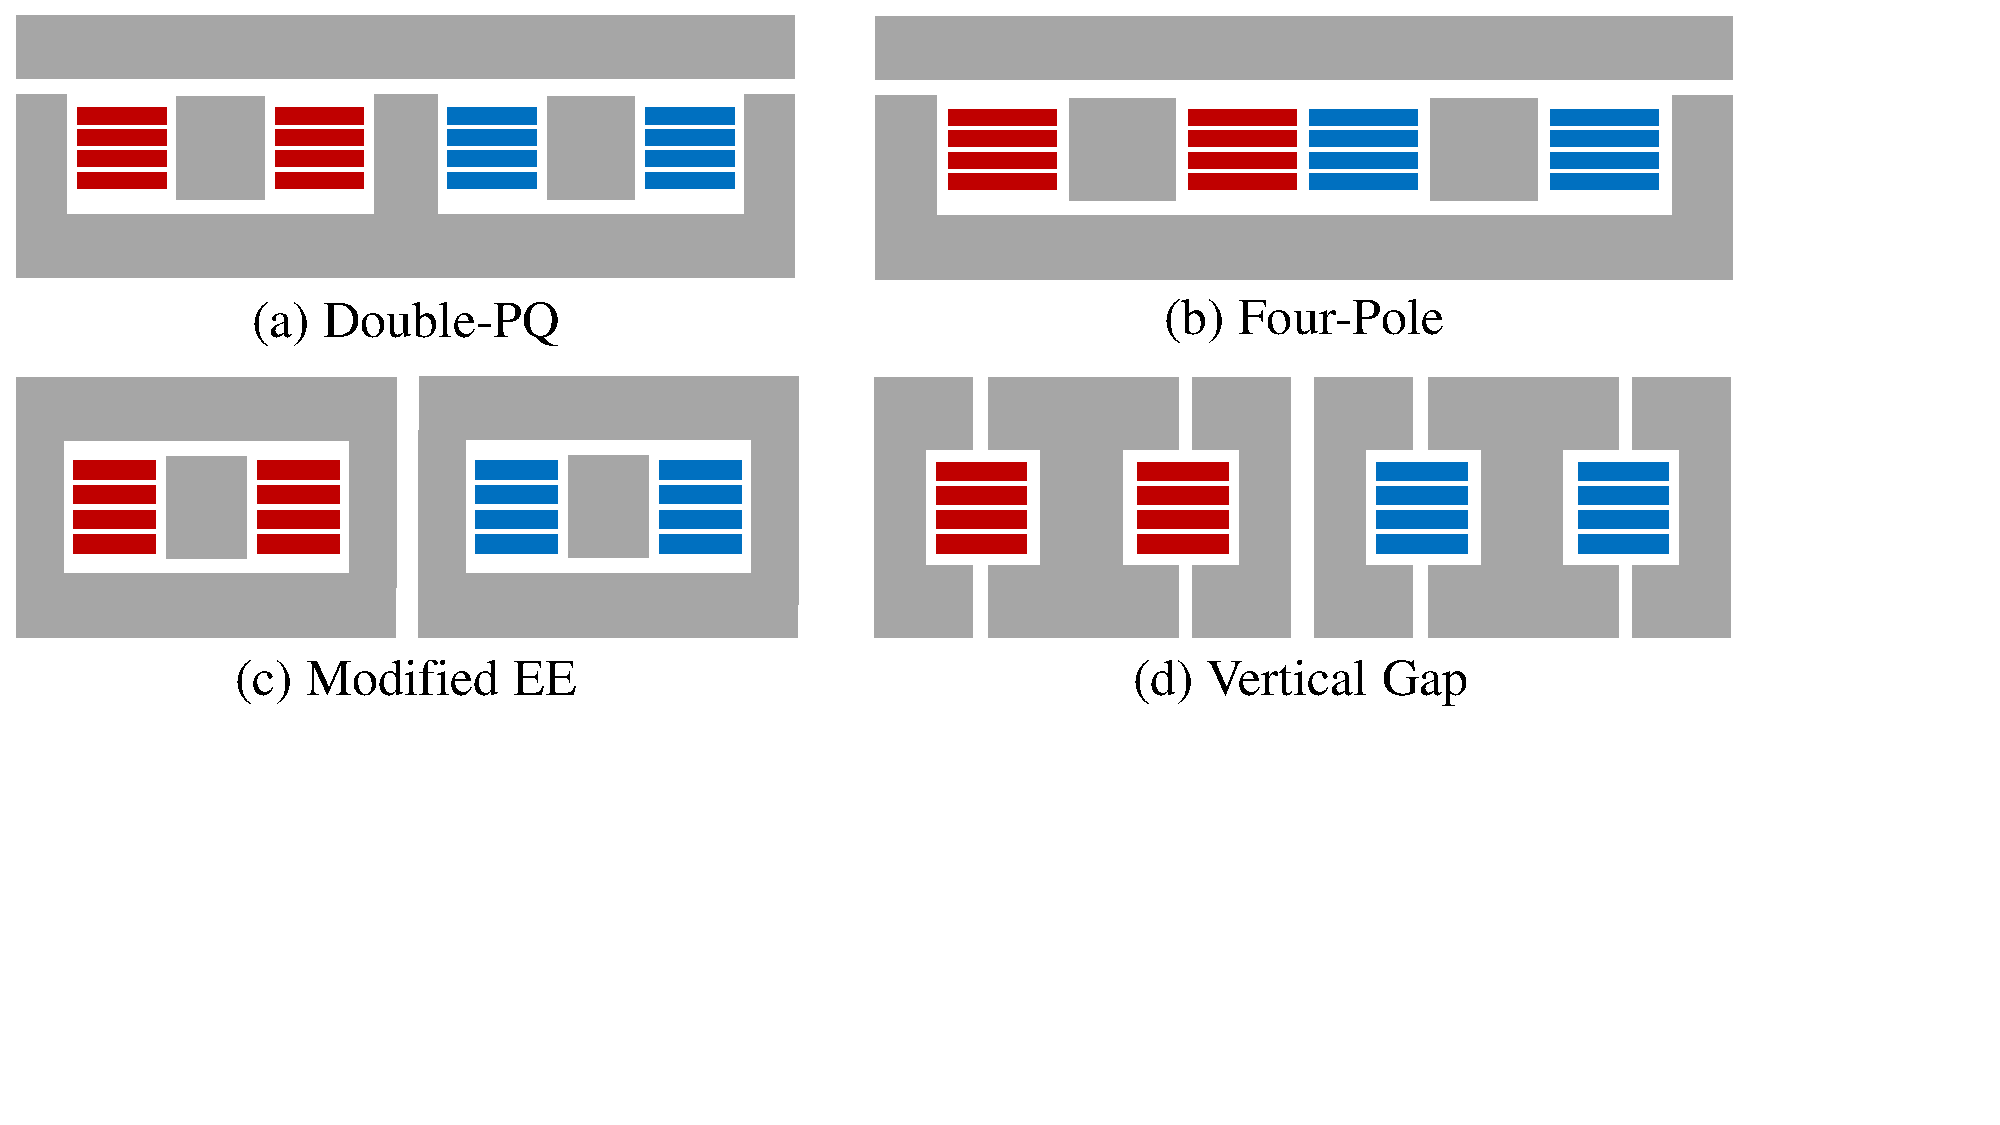
\includegraphics[page=1, trim = 0cm 7cm 4.5cm 0cm, clip, width=\columnwidth]{figures/IPEC_Figures_PowerPoint.pdf}
  \caption{Structure of the cores; Cut through the center, sie-view. First winding in red, second winding in blue.}
  \label{fig:Core_Drawings}
\end{figure}
Four different geometries, two coupled, and two uncoupled ones for reference, were considered for this application as shown in figure \ref{fig:Core_Drawings}. The Double-PQ structure was originally introduced by \cite{wangPCBWindingBasedCoupled2023}. The four-pole structure is very similar but omits the central pole which creates separate paths for DC and fundamental flux \cite{huaUltrathinCoupledInductor2021}. Both of these geometries were previously used with a two-piece core that only has air-gaps at the top. The dual air-gaps are introduced here. The third geometry is basically an EE-Core but instead of one central gap two gaps are used. Lastly, a vertical gap geometry is investigated which can partly compensate the internal proximity effect \cite{schaferNovelHighlyEfficient2020}. %A notable downside of the vertical gap is that it prohibits cooling with conductive materials from the top and bottom, which is usually a big advantage of planar inductors, due to the external flux in this area. 
\par All designs use a single turn with all six layers in parallel. Six layers were chosen due to the significantly cheaper manufacturing cost compared to higher layer counts. The inner layers have a thickness of \qty{70}{\um} while the outer ones have only \qty{35}{\um}, due to the tight spacing of the selected gate-driver which required a \qty{35}{\um} outer layer at the selected manufacturer to meet clearance constraints. Designs with more than one turn were not considered because the desired inductance and coupling-factor could not be achieved in that case due to fringing.

\subsection{Material limitations}
High-frequency ferrite materials for power applications have some unique properties that differ from those for lower frequency applications. TDK's PC200 was selected for this design as it exhibits very low loss in the range of \qtyrange{1}{4}{\MHz}. However, the performance of PC200 significantly degrades for a field strength $\sbl{Hdc} > \qty{50}{A/m}$ and at $\sbl{Hdc} > \qty{100}{A/m}$ its losses double \cite{tdkHighFrequencyLowLossFerrite}. Therefore, the inductor was designed with a maximum \sbl{Hdc} of \qty{40}{A/m} to have some margin.

\subsection{Positive vs negative coupling}
From figure \ref{fig:OutputAndLegRipple} there is no clear winner between positive and negative coupling. From the point of inductor design however, there is a very notable difference in the DC-flux distribution: For negative coupling, it is distributed very uniformly across the core resulting in a low peak field strength. For positive coupling, the DC-flux circulates between the two pillars resulting in a large imbalance in DC-flux between the inner and outer part of the core as shown in figure \ref{fig:Fluxposneg}. The peak field strength is much higher and as the core has to be designed with respect to the \sbl{Hdc} limit, this means thick top and bottom even though this area is not needed on the outside. As a result, the core gets much larger without having a performance improvement. Therefore, negative coupling is clearly the better choice. \par  

\begin{figure}
  \includegraphics[page=3, trim = 0cm 1cm 3.5cm 0cm, clip, width=\columnwidth]{figures/IPEC_Figures_PowerPoint.pdf}
  \caption{Flux-Distribution for negative and positive coupling for a DC phase current of \qty{40}{\A} and \qty{100}{\A} of ripple. With negative coupling, the two windings generate an opposing magnetomotive force for DC resulting in a low flux and relatively uniform distribution. For positive coupling, the two magnetomotive forces are driving a DC-flux in the same direction causing a large flux that only circulates between the two windings. For the fundamental, the flux-regions are swapped.}
  \label{fig:Fluxposneg}
\end{figure}

\subsection{Simulation Process}
For the simulation, the open-source 2D FEM software FEMM was used due to its high speed and easy integration with Matlab. As the core-structures are neither planar nor axisymmetric, the designs were first transformed to a planar structure. All cross-sectional areas are kept the same and the depth of the design is determined by the length of the winding\footnote{As the current does not flow in the middle of the winding but closer to its center due to the shorter length and the magnetic field, the circumference taken not from the middle of the winding but closer to the inside}. \\
For validation, the design was also transformed into an axisymmetric structure (neglecting the effects of coupling). This has the advantage that the current distribution and consequently copper-loss is closer to reality at the expense of less-precise core-loss.

\subsection{Split air-gap and optimized windings}
\begin{figure}
  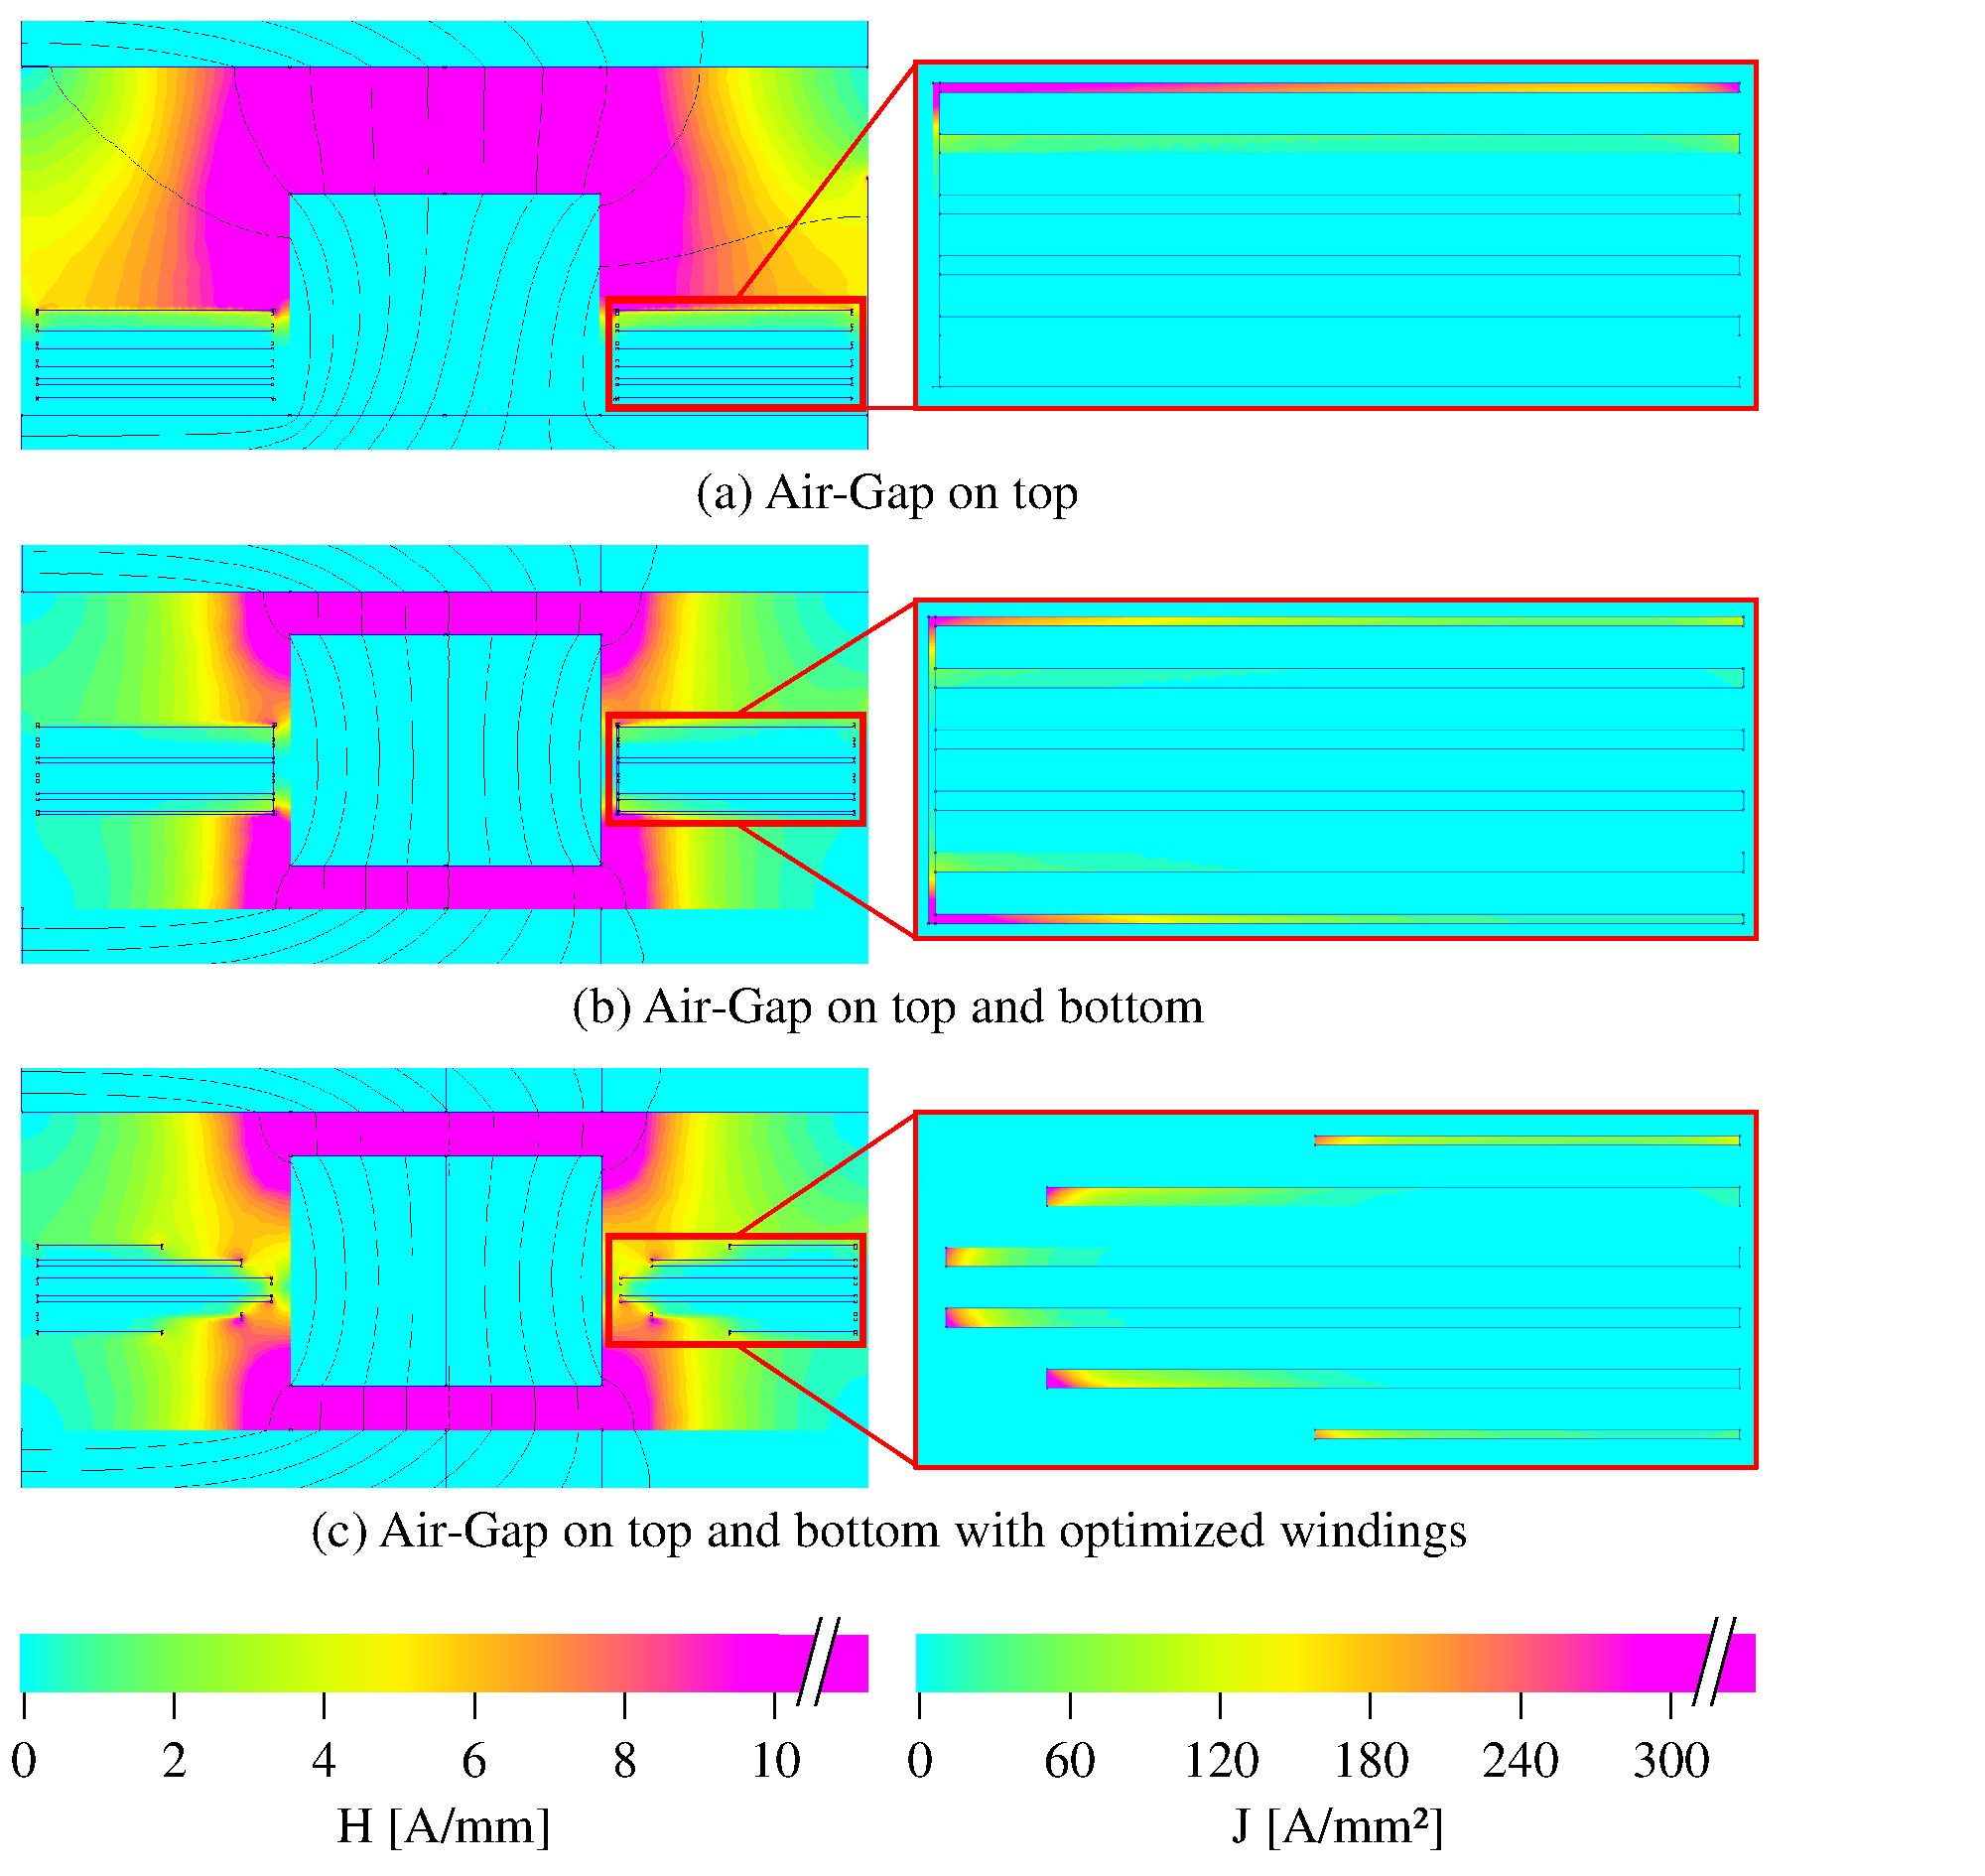
\includegraphics[page=1, trim = 0cm 0cm 3cm 0cm, clip, width=\columnwidth]{figures/IPEC_Figure_AirGap.pdf}
  \caption{Field and current distribution for different approaches. Because all layers are in parallel the current crowds in areas of large H. By splitting the gap, the field gets distributed more evenly and the current distribution improves. Utilizing a smaller width for the outer layers, i.e. moving the copper away from the high-flux areas distributes the current even better.}
  \label{fig:OptimizedGap}
\end{figure}

\begin{table}
  \centering
  \caption{Comparison of the size and loss of the optimized pillar and windings for the four-pole design.}
    \begin{tabular}{|p{0.35\columnwidth}|p{0.2\columnwidth}|p{0.25\columnwidth}|}
    \hline  
      & {Volume [\unit{\cubic\cm}]} & {Copper Loss [\unit{\W}]} \\
    \hline
    \hline
    Original design & 5.8 & 7.0 \\
    \hline
    Air-Gap on top and bottom & 5.5 & 5.7 \\
    \hline
    Air-Gap on top and bottom, curved windings & 5.3 & 5.0 \\
    \hline
    \end{tabular}%
  \label{tab:OptimizationPQ}%
\end{table}%

The external proximity effect caused by the air-gap plays an important role for the current distribution and consequently the losses of this high-frequency inductor. The field-strength at the top of the windings is large and almost zero at the bottom. As a result, the AC current is only flowing in the top layers. By centering the pillar vertically in the window such that there is an equal air-gap on the top and on the bottom, the field-strength is distributed much more uniformly and current flows in the top and bottom layers. This results in a \qty{20}{\percent} reduction in losses, which can be reduced even further by using curved windings as shown in table \ref{tab:OptimizationPQ}.

\subsection{Inductor Design Process}
Using a brute-force algorithm was deemed impossible due to the many free variables with the custom design. Instead, a manual optimization was conducted for each structure. The desired switching-frequency was fixed to \qty{1.5}{\MHz} for full-load operation, the coupling-factor to -0.3, and the winding with to \qty{3}{\mm} as this showed a good balance between size and losses. The cross-sectional areas were designed to result in $\sbl{Hdc} \leq \qty{40}{\A\per\m}$ and the air-gaps are defined by desired inductance (i.e. switching frequency) and coupling-factor. The spacing between \ac{pcb} and top/bottom of the core is the only free variable and has to be chosen for a compromise between size and efficiency.

\begin{figure}
  \centering
  % This file was created by matlab2tikz.
%
\definecolor{mycolor1}{rgb}{0.00000,0.44700,0.74100}%
%
\begin{tikzpicture}

\begin{axis}[%
width=0.8\columnwidth,
height=0.35\columnwidth,
at={(0\columnwidth,0\columnwidth)},
scale only axis,
xmin=0.2,
xmax=2,
xlabel style={font=\color{white!15!black}},
xlabel={Spacing [mm]},
ymin=4.5,
ymax=7.5,
ylabel style={font=\color{white!15!black}},
ylabel={Copper-Loss [W]},
axis background/.style={fill=white},
xmajorgrids,
ymajorgrids
]
\addplot [color=mycolor1, mark=o, mark options={solid, mycolor1}, forget plot]
  table[row sep=crcr]{%
0.2	7.13296642485744\\
0.4	6.24346547710337\\
0.6	5.71549329037772\\
0.8	5.37601200977181\\
1	5.15029927094516\\
1.2	5.00087651688349\\
1.4	4.89772868492222\\
1.6	4.83930849566333\\
1.8	4.80515358408807\\
2	4.7881839177051\\
};
\addplot[mark=*] coordinates {(1.2, 5.00087651688349)} node[pin=30:{Design point}]{} ;
\end{axis}
\end{tikzpicture}%
  \caption{Spacing between PCB and core vs. loss for the four-pole core (with curved windings and centered pillar). The distance between the PCB and the side air-gap core is fixed to \qty{0.2}{\mm} and the distance between PCB and bottom is varied. The pillar is always centered between top and bottom.}
  \label{fig:fourPole_spacingVsLoss}
\end{figure}

\subsection{Vertical Air-Gap}
The design with vertical air-gap showed a significantly lower loss compared to a traditional horizontal gap while having a much lower volume. This confirms the results from \cite{schaferNovelHighlyEfficient2020}. The main downside of this design is the significant external field on top and bottom of the inductor. This makes cooling difficult as no conductive material can be placed on top or bottom of the core, eliminating one of the typical advantages of planar inductors: The large area for cooling. Cooling from the side is proposed by \cite{schaferNovelHighlyEfficient2020} by having copper extending to the outside of the core where a heatsink can be attached but this is much less convenient and requires additional space.

\subsection{Comparison of Core Structures}
A comparison of the core structures is shown in table \ref{tab:InductorComparison}. All designs except the one with vertical gap use the optimized curved windings. The four-pole structure showed the lowest losses and and volume.
\begin{table}
  \centering
  \caption{Comparison of the size and loss of the different core structures for \qty{1.5}{\MHz} respecting the \sbl{Hdc} limit.}
    \begin{tabularx}{\columnwidth}{|l|X|X|X|X|}
      \hline
          & {Total Area [\unit{\cm\squared}]} & {Height [\unit{\cm}]} & {Volume [\unit{\cubic\cm}]} & {Copper Loss [\unit{\W}]} \\
      \hline
      \hline
      Four-Pole & 5.5 & 0.9 & 5.3 & 5.0 \\
      \hline
      Double PQ & 6.2 & 0.9 & 5.5 & 5.2 \\
      \hline
      Vertical gap & 8.0 & 0.7 & 5.8 & 5.6 \\
      \hline
      UU core & 8.1 & 1.1 & 8.9 & 6.0 \\
      \hline
    \end{tabularx}%
  \label{tab:InductorComparison}%
\end{table}%

\section{Experimental prototype}
\subsection{Hardware implementation}
\begin{figure}
  \centering
  \includegraphics[page=2, trim = 0cm 0cm 3cm 0cm, clip, width=\columnwidth]{figures/IPEC_Figures_PowerPoint.pdf}
  \caption{Fully assembled prototype (without heatspreader).  The converter area shown in orange is 45 x 29 x \qty{9.5}{\mm}. Outside of this area only the connectors for power and programming are placed as well as a protection diode and the programming resistors.}
  \label{fig:PrototypePicture}
\end{figure}
The assembled prototype is shown in figure \ref{fig:PrototypePicture}. The boxed volume of just \qty{12.4}{\cubic\cm} results in a power density of \qty{80}{\kW\per\liter} (\qty{1300}{\W\per\cubic\inch}) 
It uses Infineon's IGC025S08S1 \qty{80}{\V} GaN HEMTs and Analog Devices' LT8418 gate drivers. Two parallel low side transistors per phase are used as the converter operates at a low dutycycle. To minimize the stray inductance, the decoupling capacitors for the half-bridges were connected to the devices with a vertical power-loop layout which uses the first inner layer as a return path as proposed by \cite{reuschUnderstandingEffectPCB2014}.
The whole system is controlled by a TI F280049C real-time microcontroller. Furthermore, the TPSM365R6 integrated buck-converter module is used for the housekeeping power-supply and an Allegro Microsystems ACS37220 monitors the input current.
A total of 44 \qty{2.2}{\uF} 0805 \qty{100}{\V} X7R capacitors are used to stabilize the input voltage resulting in a derated input capacitance of \qty{20}{\uF}. This relatively small package was chosen because larger packages exhibit too much inductance causing resonance in the capacitor. At the output, 16 capacitors of the same type with a derated capacitance of \qty{33}{\uF} are used to provide a low-ripple output voltage. Compared to other designs, this converter does not need any additional off-board capacitance.


\subsection{Test results}
The converter operates over the entire range as expected. The efficiency is shown in figure \ref{fig:Efficiency} which reaches its maximum of \qty{96.3}{\percent} at around \qty{550}{\W}, demonstrating the efficacy of the inductor structure.

A more detailed analysis of the losses will be given in the final paper including a calculated contribution of the dielectric volume loss as introduced by \cite{baumannInvestigationCorelossMechanisms2022}. 

\begin{figure}
  \centering
  %% Matlab Colors
\definecolor{mycolor1}{rgb}{0.00000,0.44700,0.74100}%
\definecolor{mycolor2}{rgb}{0.85000,0.32500,0.09800}%
\definecolor{mycolor3}{rgb}{0.92900,0.69400,0.12500}%
\definecolor{mycolor4}{rgb}{0.49400,0.18400,0.55600}%
\definecolor{mycolor5}{rgb}{0.46600,0.67400,0.18800}%
\definecolor{mycolor6}{rgb}{0.30100,0.74500,0.93300}%

\begin{tikzpicture}
    \begin{axis}[%
        axis y line*=left,
        width=\columnwidth,
        height=0.6\columnwidth,
        xmin=0,
        xmax=1000,
        ymin = 0.9,
        ymax = 0.98,
        xlabel={\sbl{Pout} [W]},
        ylabel={Efficiency},
        yticklabel={\pgfmathparse{\tick*100}\pgfmathprintnumber{\pgfmathresult}\%},
        xmajorgrids,
        xminorgrids,
        minor x tick num=1,
        ymajorgrids,
        yminorgrids,
        minor y tick num=1,
        legend style={at={(0.5,-0.3)}, anchor=north, legend cell align=left, align=left, draw=white!15!black},
        legend columns=3,
        cycle list name=mark list*
    ]
        \addplot+ [smooth, color=mycolor1, mark options={solid, mark size=1.5pt, mycolor1}]
        table[row sep=crcr]{%
62.9	0.691694257\\
125.5	0.815818548\\
188.0	0.867678959\\
250.2	0.896092267\\
312.2	0.913584221\\
373.9	0.925145996\\
435.3	0.93331475\\
496.4	0.939204148\\
557.1	0.943657677\\
617.3	0.946993756\\
676.9	0.949462788\\
735.9	0.951215098\\
794.0	0.952391805\\
850.7	0.953146007\\
905.1	0.953529288\\
954.3	0.953652443\\
997.8	0.952362317\\
1039.1	0.948949772\\
        };
        \addlegendentry{\qty{1.25}{\MHz}}

        \addplot+ [smooth, color=mycolor2, mark options={solid, mark size=1.5pt, mycolor2}]
        table[row sep=crcr]{%
61.7	0.742108935\\
123.1	0.85041111\\
184.2	0.893615989\\
245.0	0.916766467\\
305.3	0.93057418\\
365.3	0.939723701\\
424.7	0.946047092\\
483.5	0.950520936\\
541.7	0.953613238\\
598.6	0.955864976\\
653.7	0.957448367\\
704.7	0.958501088\\
749.6	0.95826356\\
792.8	0.955006505\\
829.8	0.948969556\\
        };
     \addlegendentry{\qty{1.5}{\MHz}}

        \addplot+ [smooth, color=mycolor3, mark options={solid, mark size=1.5pt, mycolor3}]
        table[row sep=crcr]{%
62.1	0.808207945\\
123.7	0.892705101\\
184.8	0.924369748\\
245.2	0.940517737\\
305.0	0.950394167\\
363.6	0.95630787\\
420.3	0.960332694\\
473.4	0.963192056\\
520.6	0.963357083\\
565.4	0.958645597\\
604.5	0.949556994\\
640.3	0.942556825\\
        };
        \addlegendentry{\qty{2}{\MHz}}

        \addplot+ [smooth, color=mycolor4, mark options={solid, mark size=1.5pt, mycolor4}]
        table[row sep=crcr]{%
59.5	0.841743314\\
118.1	0.911878282\\
175.6	0.937486654\\
231.5	0.950322289\\
284.5	0.958559348\\
331.7	0.96159309\\
375.4	0.955384185\\
414.1	0.942270059\\
442.7	0.927589675\\
        };
        \addlegendentry{\qty{2.5}{\MHz}}

        \addplot+ [smooth, color=mycolor5, mark options={solid, mark size=1.5pt, mycolor5}]
        table[row sep=crcr]{%
57.2	0.856371361\\
112.7	0.920470319\\
165.5	0.943988136\\
212.8	0.95387305\\
255.4	0.94690003\\
293.2	0.927676538\\
316.8	0.902598143\\
        };
        \addlegendentry{\qty{3}{\MHz}}

        \addplot+ [smooth, color=mycolor6, mark=none]
        table[row sep=crcr]{%
213.23	0.95387305\\
332.12	0.96159309\\
520.87	0.9634\\
749.68	0.9583\\
954.41	0.953652443\\
        };
        \addlegendentry{Max}

\end{axis}
\end{tikzpicture}%
  \caption{Efficiency.}
  \label{fig:Efficiency}
\end{figure}

\bibliographystyle{IEEEtran}
\bibliography{Paper_Bibliography}

\end{document}

% https://ipec2026.org/regular-session/ 

% The extended summary should clearly define the salient concepts
% and novel features of the work. Be sure to mention past or
% previous works to distinguish your originality from them. The
% extended summary should be up to 4 pages except Reference,